% Sandia National Laboratories is a multimission laboratory managed and
% operated by National Technology & Engineering Solutions of Sandia, LLC, a
% wholly owned subsidiary of Honeywell International Inc., for the U.S.
% Department of Energy’s National Nuclear Security Administration under
% contract DE-NA0003525.

% Copyright 2002-2019 National Technology & Engineering Solutions of Sandia,
% LLC (NTESS).

%%-------------------------------------------------------------------------
%% Purpose        : Main LaTeX Xyce Users' Guide
%% Special Notes  : Graphic files (pdf format) work with pdflatex.  To use
%%                  LaTeX, we need to use postcript versions.  Not sure why.
%% Creator        : Scott A. Hutchinson, Computational Sciences, SNL
%% Creation Date  : {05/23/2002}
%%
%%-------------------------------------------------------------------------

\chapter{Analysis Types}
\label{Analysis_Chap}

\chapteroverview{Chapter Overview}
{
This chapter describes the different analysis types
available in \Xyce{}.  It includes the following sections:
\begin{XyceItemize}
\item Section~\ref{analysis_intro},     {\em Introduction}
\item Section~\ref{DC_Analysis},        {\em DC Analysis}
\item Section~\ref{Transient_Analysis}, {\em Transient Analysis}
\item Section~\ref{STEP_Analysis},      {\em STEP Parametric Analysis}
\item Section~\ref{SAMPLING_Analysis},  {\em Sampling Analysis}
\item Section~\ref{HB_Analysis},        {\em Harmonic Balance Analysis}
\item Section~\ref{AC_Analysis},        {\em AC Analysis}
\item Section~\ref{NOISE_Analysis},     {\em Noise Analysis}
\item Section~\ref{SENS_Analysis},      {\em Sensitivity Analysis}
\item Section~\ref{SP_Analysis},        {\em S-parameter Analysis}
\end{XyceItemize}
}

\section{Introduction}
\label{analysis_intro}

\Xyce{} supports several simulation analysis options, including DC bias point (\texttt{.DC}, section~\ref{DC_Analysis}), transient
(\texttt{.TRAN}, section~\ref{Transient_Analysis}), AC (\texttt{.AC}, section~\ref{AC_Analysis}), Noise (\texttt{.NOISE}, section~\ref{NOISE_Analysis}),
harmonic balance (\texttt{.HB}, section ~\ref{HB_Analysis}), and sensitivity (\texttt{.SENS}, section~\ref{SENS_Analysis}) analysis.
%, and multitime partial differential equation (PDE) (\texttt{.MPDE}, section~\ref{MPDE_Analysis}) analysis. 

Using \texttt{.STEP}(section~\ref{STEP_Analysis}), \Xyce{} can also apply an outer parametric loop to any type of analysis. This allows one (for example) to sweep a model parameter and perform a transient simulation for each parameter value.

Using \texttt{.SAMPLING}(section~\ref{SAMPLING_Analysis}), \Xyce{} can apply random sampling loop to any type of analysis.   This will compute statistical moments for various circuit outputs.

There are some analysis types typically found in SPICE-style simulators that are still a work in progress for \Xyce{}. Operating point analysis (\texttt{.OP}, section ~\ref{OP_Analysis}) is partially supported in \Xyce{}.

% -------------------------------------------------------------------------
% DC Analysis Section ---------------------------------------------------
% -------------------------------------------------------------------------
\section{Steady-State (.DC) Analysis}
\label{DC_Analysis}
\label{DC_Sweep_Overview}
\index{analysis!DC} \index{DC analysis}
\index{DC Sweep} \index{analysis!DC sweep}

The DC sweep analysis capability in \Xyce{} computes the DC bias point
of a circuit for a range of values of input sources.  DC sweep is
supported for a source or device parameter, through a range of
specified values.  As the sweep proceeds, \Xyce{} computes the bias
point\index{bias point} for each value in the specified range of the
sweep.

If the variable to be swept is a voltage or current source, a DC source must be
used and its value set in the netlist (see \Xyce{} Reference 
Guide\ReferenceGuide{}). In simulating the DC response of an analog
circuit, \Xyce{} eliminates time dependence from the circuit by treating capacitor elements as open circuits and inductor elements as short circuits, while using only the DC values of voltage and current sources.

\subsection{.DC Statement}

To specify a \verb|.DC| analysis, include a \verb|.DC| line in the netlist.  Some examples of typical \verb|.DC| lines are:

\Example{\\
\texttt{ .DC V1  7m 5m -1m } \\
\texttt{ .DC I1  5u 10u 1u } \\
\texttt{ .DC M1:L  7u 5u -1u } \\
\texttt{ .DC OCT V0 0.125 64 2 } \\
\texttt{ .DC DEC R1 100 10000 3 } \\
\texttt{ .DC TEMP LIST 10.0 15.0 18.0 27.0 33.0 }\\
\texttt{ .DC data=table }
}

The examples include several types of sweep --- linear, octave,
decade, list and data.  They also demonstrate sweeping over voltage and current
sources as well as device parameters.  The \Xyce{} Reference
Guide\ReferenceGuide{} provides a complete description of each.

\subsection{Setting Up and Running a DC Sweep}
\label{Running_DC_Sweep}
\index{DC sweep!running}

Following the example given in section~\ref{DC_Sweep}, figure~\ref{Clipper_Netlist3} shows the diode clipper circuit netlist with a DC sweep analysis specified.  Here, the voltage source \texttt{Vin} is swept from -10 to 15 in 1-volt increments, resulting in 26 DC operating point calculations.  

NOTE:	\Xyce{} ignores the default setting for \texttt{Vin} during these calculations.  All other source values use the specified values (in this case, \texttt{VCC =  5V}).

Running \Xyce{} on this netlist produces an output results file named
\verb|clipper.cir.prn|.  Obtaining this file requires specifying the \verb|.PRINT DC| line. Plotting this data produces the graph shown in figure~\ref{Clipper_DCSweep2}.

\begin{figure}[htbp]
\begin{centering}
\shadowbox{
\begin{minipage}{0.8\textwidth}
\begin{vquote}

Diode Clipper Circuit
** Voltage Sources
VCC 1 0 5V 
VIN 3 0 0V
* Analysis Command
\color{XyceRed}.DC VIN -10 15 1\color{black}
* Output
.PRINT DC V(3) V(2) V(4)
* Diodes
D1 2 1 D1N3940 D2 0 2 D1N3940
* Resistors
R1 2 3 1K
R2 1 2 3.3K
R3 2 0 3.3K
R4 4 0 5.6K
* Capacitor
C1 2 4 0.47u
.MODEL D1N3940 D(
+ IS=4E-10 RS=.105 N=1.48 TT=8E-7
+ CJO=1.95E-11 VJ=.4 M=.38 EG=1.36
+ XTI=-8 KF=0 AF=1 FC=.9
+ BV=600 IBV=1E-4)
.END

\end{vquote}
\end{minipage}
}
\caption{Diode clipper circuit netlist for DC sweep analysis.\label{Clipper_Netlist3}}

\end{centering}
\end{figure}

\begin{figure}[htbp]
\begin{centering}
  \shadowbox{ 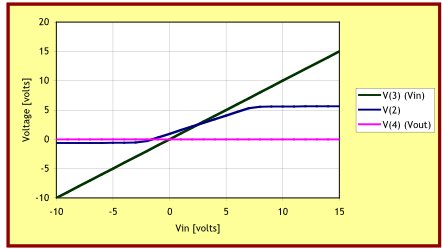
\includegraphics[width=4.5in]{clipper-dcsweep} }
\caption{DC sweep voltages at Vin, node 2 and Vout.\label{Clipper_DCSweep2}}
\end{centering}
\end{figure}

\subsection{OP Analysis}
\label{OP_Analysis}
\index{\texttt{.OP}}
\index{DC sweep!OP Analysis}
\index{OP analysis}

\Xyce{} also supports \texttt{.OP} analysis statements.  In \Xyce{}, consider \texttt{.OP} as a shorthand for a single-step DC sweep, in which all the default operating point values are used.  One may also consider
\texttt{.OP} analysis to be the operating point calculation that would occur as the initial step to a transient calculation, without the subsequent time steps.

This capability was mainly added to enable the code to handle legacy
netlists using this analysis statement type.  In most versions of
SPICE, using \texttt{.OP} results in extra output not available from a
DC sweep.  \Xyce{} will also output some of this extra information about
devices, but the capability is not fully implemented.

\subsection{Output}
\label{DC_Output}\index{\texttt{.PRINT}!\texttt{DC}}

During analysis a number of output files may be generated.  The
selection of which files are created depends on a variety of factors,
most obvious of which is the \texttt{.PRINT} command.
Table~\ref{DC_Output_table} lists the format options and files created.
The column labeled ``Additional Columns'' lists the additional data that
is written, though not specified on the \texttt{.PRINT} line.

\begin{table}[htbp]
  \caption{Output generated for DC analysis \label{DC_Output_table}}
  \begin{tabularx}{\linewidth}{|p{2.75in}|Y|Y|}
    \rowcolor{XyceDarkBlue} \color{white}\textbf{Command} & \color{white}\textbf{Files} & \color{white}\textbf{Additional Columns} \\ \hline
\texttt{.PRINT DC} & \emph{circuit-file}.prn & INDEX TIME \\ \hline
\texttt{.PRINT DC FORMAT=NOINDEX} & \emph{circuit-file}.prn & TIME \\ \hline
\texttt{.PRINT DC FORMAT=CSV} & \emph{circuit-file}.csv & TIME \\ \hline
\texttt{.PRINT DC FORMAT=RAW} & \emph{circuit-file}.raw & TIME \\ \hline
\texttt{.PRINT DC FORMAT=TECPLOT} & \emph{circuit-file}.dat & TIME \\ \hline
\texttt{.PRINT DC FORMAT=PROBE} & \emph{circuit-file}.csd & TIME \\ \hline

\texttt{\emph{Xyce} -r} & \emph{circuit-file}.raw & All circuit variables printed \\ \hline
\texttt{\emph{Xyce} -r -a} & \emph{circuit-file}.raw & All circuit variables printed \\ \hline

\texttt{.OP} & \emph{log-file} & Operating point information \\ \hline

  \end{tabularx}
%% \index{sources!time-dependent}
\end{table}





%%%%%%
% -------------------------------------------------------------------------
% Transient Analysis Section ----------------------------------------------
% -------------------------------------------------------------------------
%\clearpage
\section{Transient Analysis}
\label{Trans_Overview}
\label{Transient_Analysis}
\index{analysis!transient} \index{transient analysis}
\index{\texttt{.TRAN}}

The transient response analysis simulates the response of the circuit from
\texttt{TIME=0} to a specified time.  Throughout a transient analysis, 
any or all of the independent sources may have time-dependent values.

In \Xyce{} (and most other circuit simulators), the transient analysis begins by performing its own bias 
point\index{bias point} calculation at the beginning of the run, using the same method as used for DC sweep. This is required to set the initial conditions for the transient solution as the initial values of the 
sources may differ from their DC values.

\subsection{.TRAN Statement}

To run a transient simulation, the circuit netlist file must contain a
\verb|.TRAN| command.

\Example{\\
\texttt{ .TRAN 100us 300ms } \\
\texttt{ .TRAN 100p 12.05u 9.95u }
}

The \Xyce{} Reference Guide\ReferenceGuide{} provides a detailed explanation of the \verb|.TRAN| statement. The netlist must also contain one of the following:

\begin{XyceItemize}
\item Independent, transient source (see table~\ref{Time_Sources}),
\item Initial condition on a reactive element, or
\item Time-dependent analog behavioral modeling source (see chapter~\ref{Behavioral_Modeling})
\end{XyceItemize}

\subsection{Defining a Time-Dependent (transient) Source}
\label{Defining_Source}
\index{sources!defining time-dependent}

\subsubsection{Overview of Source Elements}

Source\index{sources} elements, either voltage or current, are entered
in the netlist\index{netlist!sources} file as described in the \Xyce{}
Reference Guide\ReferenceGuide{}.  Table~\ref{Time_Sources} lists the
time-dependent sources available in \Xyce{} for either voltage or
current.  For voltage sources, the name is preceded by \texttt{V} while
current sources are preceded by \texttt{I}.

\begin{table}[htbp]
  \caption{Summary of \Xyce{}-supported time-dependent sources \label{Time_Sources}}
  \begin{tabularx}{\linewidth}{|Y|Y|}
    \rowcolor{XyceDarkBlue} \color{white}\bf Source Element Name &
    \color{white}\bf Description \\ \hline

    EXP & Exponential Waveform \\ \hline
    PAT & Pattern Waveform \\ \hline
    PULSE & Pulse Waveform \\ \hline
    PWL & Piecewise Linear Waveform \\ \hline
    SFFM & Frequency-modulated Waveform \\ \hline
    SIN & Sinusoidal Waveform \\ \hline

  \end{tabularx}
\index{sources!time-dependent}
\end{table}

To use time-dependent or transient sources, place the source element line in the netlist and characterize the transient behavior using the appropriate parameters.  Each transient source element has a separate
set of parameters dependent on its transient behavior.  In this way, the user can create analog sources that produce sine wave, square pulse, exponential pulse, single-frequency FM, and piecewise linear (PWL) waveforms.

\subsubsection{Defining Transient Sources}

To define a transient source, select one of the supported sources: independent 
voltage or current, choose a transient source type from table~\ref{Time_Sources}, and provide the transient parameters (refer to the \Xyce{} Reference 
Guide\ReferenceGuide{} to fully define the source).

The following example of an independent sinusoidal voltage source in a
circuit netlist creates a voltage source between nodes 1 and 5
that oscillates sinusoidally between -5V and +5V with a frequency of
50 KHz.  The arguments specify an offset of -5V, a 10V amplitude, and
a 50KHz frequency, in that order.

\Example{\texttt{Vexample 1 5 SIN(-5V 10V 50K)}}


\subsection{Transient Time Steps}
\label{Time_Steps}
\index{solvers!transient} \index{time step!size}

During the simulation, \Xyce{} uses a calculated time step that is continuously
adjusted for accuracy and efficiency (see~\cite{WKHH:2000} and
~\cite{Petzold:1996}).  Calculation time step increases during periods of circuit idleness, and decreases during dynamic portions of the waveform.
\index{time step!maximum size} Users may control the maximum internal step size by specifying the step's ceiling value in the \verb|.TRAN| command (see the
\Xyce{} Reference Guide\ReferenceGuide{}).

The internal calculation time steps used might not be consistent with the user-requested
\index{output!time values} output time steps.  By default,
\Xyce{} outputs solution results at every time step it calculates.  If the user
selects output timesteps via the \verb|.OPTIONS OUTPUT| statement (see
chapter~\ref{Output}), then \Xyce{} will output results at the interval
requested, interpolating solution variables to desired output times if
necessary.


\subsection{Time Integration Methods}
\label{TransientControls}
\index{solvers!transient} \index{time step!size}
For a transient analysis, several time integration methods can be selected to solve the circuit
model's differential algebraic equations.  The following algorithms are available:

\begin{XyceItemize}
\item Variable order Trapezoidal (combines Trapezoidal and Backward Euler) 
\item Gear method, orders 1-2.
\end{XyceItemize}




You can set the \verb|method|, \verb|maxord| and \verb|minord| parameters to select the time
integration methods via a .OPTIONS line. The following table shows the possible settings for those
three parameters. (Note: Consult the \Xyce{} Reference Guide\ReferenceGuide for the exact syntax of the .OPTIONS
line for each time integration method.) The default time integration method in \Xyce{} is Trap, which 
is the same as SPICE, PSpice and HSPICE.

\begin{table}[htbp]
  \caption{Summary of \Xyce{}-supported time integration methods \label{Time_integration}}
  \begin{tabularx}{\linewidth}{|Y|Y|Y|}
    \rowcolor{XyceDarkBlue} \color{white}\bf  Integration Methods &
    \color{white}\bf  Option Settings & \color{white}\bf Comments \\ \hline
    Backward-Euler & method=trap maxord=1 & Backward-Euler only \\ \hline
    Trap & method=trap & combines Trapezoidal and Backward Euler (default) \\ \hline
    Trap only & method=trap minord=2 & Trapezoidal only \\ \hline
    Gear &  method=gear &  combines Backward Euler and 2nd order Gear \\ \hline
    Gear2 only &  method=gear minord=2 & 2nd order Gear only  \\ \hline
  \end{tabularx}
\index{Time integration!integration method}
\index{\texttt{.OPTIONS}!\texttt{TIMEINT}!\texttt{METHOD}} \index{\texttt{.OPTIONS}!\texttt{TIMEINT}!\texttt{MINORD}} 
\end{table}



The Trapezoidal method is often the preferred method because it is accurate and fast.
However, this method can exhibit artificial point-to-point ringing, which can be
controlled by using tighter tolerances. If a circuit fails to converge with the
Trapezoidal method then you can re-run the transient analysis using the Gear method. 

The Gear method may help convergence for some circuits. The 2nd order Gear method is 
typically more accurate than the Backward-Euler method (1st order Gear). However, 
both of these methods are overly stable methods, and they 
can damp the actual circuit behavior when simulating high-Q resonators such as oscillators. 
The Backward-Euler method has more damping effect than the 2nd order Gear method. 
This effect can be alleviated by using tighter tolerances in the simulations. However, it is 
suggested to use the pure Trapezoidal method for oscillators.

\subsection{Error Controls}
\label{Time_Step_Selection}
\index{solvers!transient} \index{time step!size} \index{time step!how to select}

There are two basic  time-step error control methods in \Xyce{} --- Local
Truncation Error (LTE) based and non-LTE based.  


\subsubsection{Local Truncation Error (LTE) Strategy}
\index{\texttt{.OPTIONS}!\texttt{TIMEINT}!\texttt{RELTOL}} \index{\texttt{.OPTIONS}!\texttt{TIMEINT}!\texttt{ABSTOL}}
All time integration methods use the LTE-based strategy by default. The
accuracy of the simulation can be controlled by specifying appropriate relative
and absolute error tolerances (RELTOL and ABSTOL).

\Example{\\
\texttt{ .OPTIONS TIMEINT RELTOL=1e-4 ABSTOL=1e-8 } \\
}

The total tolerance of LTE is
{\\
\texttt{ $Tol_{LTE}$  = abstol +  reltol*ref}  
}

The parameter \verb|ref| is the reference value that the relative error is compared to. It can be controlled by setting \verb|newlte| option.
\index{\texttt{.OPTIONS}!\texttt{TIMEINT}!\texttt{NEWLTE}}
\Example{\\
\texttt{ .OPTIONS TIMEINT NEWLTE=1 } \\
}

The  choices for \verb|newlte| option are:

\begin{XyceItemize} 
\item 0. The reference value is the current value on each node. This is the most conservative and least used.
\item 1. The reference value is the maximum of all the signals at the current time. This is the default value.
\item 2. The reference value is the maximum of all the signals over all past time. This is the loosest criterion. It normally produces the best performance and should be used if the overall size of the signals is roughly the same on all nodes.
\item 3. The reference value is the maximum value on each signal over all past time. This should be used if the scale of signals varies widely in a system.
\end{XyceItemize}

The Trapezoid integrator algorithm introduces no numerical dissipation.  So,
a strong ringing (artificially introduced by the numerical algorithm) will
occur when sources or models introduce discontinuities.  This can result in a
large local truncation error estimate, ultimately leading to a ``time-step too
small'' error.  In this case, using the Gear method or a non-LTE
strategy may help.

\subsubsection{Non-LTE Strategy}
The non-LTE strategy used in \Xyce{} is based on success of the nonlinear solve, and is enabled by setting ERROPTION=1.  Since the step-size selection is based only upon nonlinear iteration statistics rather than accuracy, it is highly suggested that DELMAX be specified, in a circuit-specific manner, for all three time integrators.  The purpose of DELMAX is to limit the largest time step taken.

\Example{\\
\texttt{ .OPTIONS TIMEINT ERROPTION=1 DELMAX=1.0e-4 } \\
}

For the Trapezoid and Gear integrators, the options are slightly more refined.  If the number of nonlinear iterations is below NLMIN, then the step size is doubled. If the number of nonlinear iterations is above NLMAX then the step size is cut by one eighth.  In between, the step size is not changed.  An example using Trap (METHOD=7) is given below. 
\index{\texttt{.OPTIONS}!\texttt{TIMEINT}!\texttt{NLMIN}} \index{\texttt{.OPTIONS}!\texttt{TIMEINT}!\texttt{NLMAX}} \index{\texttt{.OPTIONS}!\texttt{TIMEINT}!\texttt{DELMAX}}

\Example{\\
\texttt{ .OPTIONS TIMEINT METHOD=7 ERROPTION=1 NLMIN=3 NLMAX=8 DELMAX=1.0e-4 } \\
}

If the number of Newton iterations is bigger than NLmax and TIMESTEPSREVERSAL is not set, then \Xyce{} will cut the next step.  If the number of Newton iterations is bigger than NLmax and  TIMESTEPSREVERSAL is set, then \Xyce{} will reject the current step and also cut the current step.

\Example{\\
\texttt{ .OPTIONS TIMEINT METHOD=7 ERROPTION=1 DELMAX=1.0e-4 TIMESTEPSREVERSAL=1 } \\
}

\subsection{Breakpoints}

\index{\texttt{.OPTIONS}!\texttt{TIMEINT}!\texttt{BREAKPOINTS}} 

It is often necessary or desirable for the time integrator to be forced to land on a specific time point 
and restart integration from that point.   The most common scenario for which this is necessary is when
an device (such as a \texttt{PULSE} or a \texttt{PWL} source) produces a discontinuity.  If a discontinuity is
present, and no breakpoint is set, then the LTE analysis will force the time integrator to take really small
time steps, and this can possibly impact the robustness of the calculation.

Fortunately, \Xyce{} handles most device-based discontinuities automatically, so it is not necessary for the 
user to worry about them.  However, it can be desirable for the user to manually set breakpoints from the netlist.
In a \Xyce{} netlist, these are specified using the BREAKPOINTS parameter with a comma-separated list in
the following \texttt{.OPTIONS TIMEINT} statement.

\Example{\\
\texttt{ .OPTIONS TIMEINT BREAKPOINTS=1ms,2ms,3ms} \\
}

\subsection{Checkpointing and Restarting}
\label{Restart}
\index{checkpoint} \index{restart}

\Xyce{} was designed to simulate large, complex circuits over long
simulation runs.  Because complex simulations can take many hours (or
even days) to complete, it can sometimes be helpful to use
``checkpointing.''  When checkpointing is used, \Xyce{} periodically
saves its complete simulation state.  The saved state can be used to
restart \Xyce{} from one of these ``checkpoints.''  In the event of a
computer crash, power outage, or should the simulation need to be
interrupted for some other reason, checkpointing allows the user to
restart a long simulation in the middle of a run without having to
start over.

\Xyce{} uses the \index{netlist!restart} \index{\texttt{.OPTIONS}!\texttt{RESTART}} \verb|.OPTIONS RESTART|
netlist command to control all checkpoint output and restarting.  

\subsubsection{Checkpointing Command Format}
\index{checkpoint!format} \index{restart!format} \index{\texttt{.OPTIONS}!\texttt{RESTART}}

\begin{XyceItemize}
\item \verb+.OPTIONS RESTART [PACK=<0|1>] JOB=<job name> INITIAL_INTERVAL=<interval>+ \\
  \verb+[[<t0> <i0> [<t1> <i1>...]]]+

  \texttt{PACK=<0|1>} indicates whether restart data files will contain byte-packed (binary) data(\texttt{PACK=1}, the default) or unpacked (ASCII)(\texttt{PACK=0}).
  \texttt{JOB=<job name>} identifies the prefix for restart files.  The actual restart files will be the job name appended with the current simulation time (e.g., \texttt{name1e-05} for \texttt{JOB=name} and simulation time 1e-05 seconds).  Furthermore, the\\ \texttt{INITIAL\_INTERVAL=<interval>} identifies the initial interval time used for restart output; this parameter must be given.  The \texttt{<tx ix>} intervals identify times (\texttt{tx}) at which the output interval (\texttt{ix}) will change.  This functionality is identical to that described for the \index{\texttt{.OPTIONS}!\texttt{OUTPUT}}
  \texttt{.OPTIONS OUTPUT} command (section~\ref{Output_Control}).
\item Example --- Generate checkpoints every 0.1 $\mu s$:
\begin{vquote}
.OPTIONS RESTART JOB=checkpt INITIAL_INTERVAL=0.1us
\end{vquote}
\item Example --- Generate unpacked checkpoints every 0.1 $\mu s$:
\begin{vquote}
.OPTIONS RESTART PACK=0 JOB=checkpt INITIAL_INTERVAL=0.1us
\end{vquote}
\item Example --- Initial interval of 0.1 $\mu s$, at 1 $\mu s$ in the
  simulation, change to interval of 0.5 $\mu s$, and at 10 $\mu s$ change to an
  interval of 0.1 $\mu s$:
\begin{vquote}
.OPTIONS RESTART JOB=checkpt INITIAL_INTERVAL=0.1us 1us 0.5us
+ 10us 0.1us
\end{vquote}
\end{XyceItemize}

\subsubsection{Restarting Command Format}
\index{restart!format}

\begin{XyceItemize}
\item \index{\texttt{.OPTIONS}!\texttt{RESTART}}
\verb+.OPTIONS RESTART <FILE=<filename> | JOB=<job name> START_TIME=<time>>+ \\
\verb|+ [INITIAL_INTERVAL=<interval> [<t0> <i0> [<t1> <i1> ...]]]|
\end{XyceItemize}
To restart\index{restart} from an existing restart file, specify the file by using either the\\%
\texttt{FILE=<filename>} parameter to explicitly request a file or\\%
\texttt{JOB=<job name> START\_TIME=<time>} to specify a file prefix and a
specific time.  The time must exactly match an output file time for the
simulator to correctly load the file.  

To continue checkpointing the simulation in a restarted run, append
\texttt{INITIAL\_INTERVAL=<interval>} and the following intervals to
the command in the same format as previously described.  Without these
additional parameters, the simulation will restart as requested, but
will not generate further checkpoint files.

\begin{XyceItemize}
\item Example\index{Example!restarting} --- Restart from checkpoint file at 0.133
  $\mu s$:
\begin{vquote}
.OPTIONS RESTART JOB=checkpt START_TIME=0.133us
\end{vquote}
\item Example --- Restart from checkpoint file at 0.133 $\mu s$ :
\begin{vquote}
.OPTIONS RESTART FILE=checkpt0.000000133
\end{vquote}
\item Example --- Restart from 0.133 $\mu s$ and continue checkpointing at 0.1
      $\mu s$ intervals:
\begin{vquote}
.OPTIONS RESTART FILE=checkpt0.000000133 JOB=checkpt_again
+ INITIAL_INTERVAL=0.1us
\end{vquote}
\end{XyceItemize}
\subsection{Output}
\label{Transient_Output}\index{\texttt{.PRINT}!\texttt{TRAN}}

During analysis a number of output files may be generated.  The
selection of which files are created depends on a variety of factors,
most obvious of which is the \texttt{.PRINT} command.
Table~\ref{Tran_Output_table} lists the format options and files
created.  The column labeled ``Additional Columns'' lists the additional
data that is written, though not specified on the \texttt{.PRINT} line.

\begin{table}[htbp]
  \caption{Output generated for Transient analysis \label{Tran_Output_table}}
  \begin{tabularx}{\linewidth}{|p{2.75in}|Y|Y|}
    \rowcolor{XyceDarkBlue} \color{white}\textbf{Command} & \color{white}\textbf{Files} & \color{white}\textbf{Additional Columns} \\ \hline
\texttt{.PRINT TRAN} & \emph{circuit-file}.prn & INDEX TIME \\ \hline
\texttt{.PRINT TRAN FORMAT=NOINDEX} & \emph{circuit-file}.prn & TIME \\ \hline
\texttt{.PRINT TRAN FORMAT=CSV} & \emph{circuit-file}.csv & TIME \\ \hline
\texttt{.PRINT TRAN FORMAT=RAW} & \emph{circuit-file}.raw & TIME \\ \hline
\texttt{.PRINT TRAN FORMAT=TECPLOT} & \emph{circuit-file}.dat & TIME \\ \hline
\texttt{.PRINT TRAN FORMAT=PROBE} & \emph{circuit-file}.csd & TIME \\ \hline

\texttt{\emph{Xyce} -r} & \emph{circuit-file}.raw & All circuit variables printed \\ \hline
\texttt{\emph{Xyce} -r -a} & \emph{circuit-file}.raw & All circuit variables printed \\ \hline

\texttt{.OP} & \emph{log-file} & Operating point information \\ \hline

  \end{tabularx}
%% \index{sources!time-dependent}
\end{table}

% -------------------------------------------------------------------------
% STEP Analysis Section ---------------------------------------------------
% -------------------------------------------------------------------------
\clearpage
\section{STEP Parametric Analysis}
\label{STEP_Analysis}
\label{step_Overview}
\index{analysis!STEP} \index{STEP parametric analysis}
\index{\texttt{.STEP}}

The \verb|.STEP| command performs a parametric sweep for all the
analyses of the circuit.  When the \verb|.STEP| command is invoked,
typical analyses, such as \verb|.DC|, \verb|.AC|, and \verb|.TRAN| are
performed for each value of the stepped parameter.

This capability is very similar, but not identical, to the \verb|STEP| capability in 
PSpice~\cite{PSpiceUG:1998}.  
\Xyce{}  can use \verb|.STEP| to sweep over any device instance or device
model parameter, as well as the circuit temperature.  It is not legal to sweep parameters defined in \texttt{.PARAM} statements, but it is legal to sweep global parameters defined in \texttt{.global\_param} statements.  Section~\ref{Parameters_Expressions}) discusses these two distinct parameter definitions.

\subsection{.STEP Statement}

A \verb|.STEP| analysis may be specified by simply adding a \verb|.STEP| line to a netlist.  Unlike \verb|.DC|, \verb|.STEP| by itself is not an adequate analysis specification, as it merely specifies an outer loop around the normal analysis.  A standard analysis line, either specifying \verb|.TRAN|, \verb|.AC| and \verb|.DC| analysis, is still required.

Some examples of typical \verb|.STEP| lines are:

\Example{\\
\texttt{ .STEP M1:L  7u 5u -1u } \\
\texttt{ .STEP OCT V0 0.125 64 2 } \\
\texttt{ .STEP DEC R1 100 10000 3 } \\
\texttt{ .STEP TEMP LIST 10.0 15.0 18.0 27.0 33.0 } \\
\texttt{ .STEP data=table }
}

\verb|.STEP| has a format similar to that of the \verb|.DC| format
specification.  In the first example, \verb|M1:L| is the name of the
parameter (in this instance, the length parameter of the MOSFET
\texttt{M1}), \verb|7u| is the initial value of the parameter,
\verb|5u| is the final value of the parameter, and \verb|-1u| is the
step size.  Like \verb|.DC|, \verb|.STEP| in \Xyce{} can also handle
sweeps by decade, octave, a specified lists of values, or multivariate parameter values from a table.  Consult the
\Xyce{} Reference Guide\ReferenceGuide{} for complete explanations of each sweep type.

\subsection{Sweeping over a Device Instance Parameter}
\label{step_InstanceParam}

The first example uses \verb|M1:L| as the parameter, but it could have used any model or instance parameter existing in the circuit. Internally, \Xyce{} handles the parameters for all device models and device instances in the same way.  Users can uniquely identify any parameter by specifying the device instance name, followed by a colon (:), followed by the specific parameter name.  For example, all the MOSFET models have an instance parameter for the channel length, L.  For a MOSFET instance specified in a netlist, named M1, the full name for the M1 channel length parameter is M1:L.  

Figure~\ref{Step_Netlist_1} provides a simple application of \verb|.STEP| to a device instance.  This is the same diode clipper circuit as was used in the transient analysis chapter, except that a single line (in red) has been added.  This \verb|.STEP| line will cause \Xyce{} to sweep the resistance of the resistor, R4, from 3.0 KOhms to 15.0 KOhms, in 2.0 KOhms increments, meaning seven transient simulations will be performed, each one with a different value for R4.

As the circuit is executed multiple times, the resulting output file is a little more sophisticated.  The \verb|.PRINT| statement is still used in much the same way as before.  However, the .prn output file contains the concatenated output of each \verb|.STEP| increment.  The end of this section provides more details of how \texttt{.STEP} changes output files.

\begin{figure}[htbp]
\begin{centering}
\shadowbox{
\begin{minipage}{0.8\textwidth}
\begin{vquote}

Transient Diode Clipper Circuit with Step Analysis
* Voltage Sources
VCC 1 0 5V
VIN 3 0 SIN(0V 10V 1kHz)\color{black}
* Analysis Command
.TRAN 2ns 2ms\color{black}
* Output
.PRINT TRAN V(3) V(2) V(4)\color{black}
\color{XyceRed} * Step statement \color{black}
\color{XyceRed}.STEP R4:R 3.0K 15.0K 2.0K \color{black}
* Diodes
D1 2 1 D1N3940
D2 0 2 D1N3940
* Resistors
R1 2 3 1K
R2 1 2 3.3K
R3 2 0 3.3K
R4 4 0 5.6K
* Capacitor
C1 2 4 0.47u
.MODEL D1N3940 D(
+ IS=4E-10 RS=.105 N=1.48 TT=8E-7
+ CJO=1.95E-11 VJ=.4 M=.38 EG=1.36
+ XTI=-8 KF=0 AF=1 FC=.9
+ BV=600 IBV=1E-4)
.END
\end{vquote}
\end{minipage}
}
\caption{Diode clipper circuit netlist for step transient
analysis\label{Step_Netlist_1}}
\end{centering}
\end{figure}

\subsection{Sweeping over a Device Model Parameter}
\label{step_ModelParam}

Sweeping a model parameter can be done in an identical manner to an instance parameter.  Figure~\ref{Step_Netlist_2} contains the same circuit as in figure~\ref{Step_Netlist_1}, but with additional \verb|.STEP| line referring to a model parameter, \verb|D1N3940:IS|.  

NOTE:	\verb|.STEP| line syntax differs from \verb|.DC| line syntax in that multiple parameters require separate \verb|.STEP| lines. Each parameter needs a separate line.

\begin{figure}[htbp]
\begin{centering}
\shadowbox{
\begin{minipage}{0.8\textwidth}
\begin{vquote}

Transient Diode Clipper Circuit with Step Analysis
* Voltage Sources
VCC 1 0 5V
VIN 3 0 SIN(0V 10V 1kHz)\color{black}
* Analysis Command
.TRAN 2ns 2ms\color{black}
* Output
.PRINT TRAN V(3) V(2) V(4)\color{black}
\color{XyceRed} * Step statements \color{black}
\color{XyceRed}.STEP R4:R 3.0K 15.0K 2.0K \color{black}
\color{XyceRed}.STEP D1N3940:IS 2.0e-10 6.0e-10 2.0e-10 \color{black}
* Diodes
D1 2 1 D1N3940
D2 0 2 D1N3940
* Resistors
R1 2 3 1K
R2 1 2 3.3K
R3 2 0 3.3K
R4 4 0 5.6K
* Capacitor
C1 2 4 0.47u
.MODEL D1N3940 D(
+ IS=4E-10 RS=.105 N=1.48 TT=8E-7
+ CJO=1.95E-11 VJ=.4 M=.38 EG=1.36
+ XTI=-8 KF=0 AF=1 FC=.9
+ BV=600 IBV=1E-4)
.END
\end{vquote}
\end{minipage}
}
\caption{Diode clipper circuit netlist for 2-step transient
analysis\label{Step_Netlist_2}}
\end{centering}
\end{figure}

\subsection{Sweeping over Temperature}
\label{step_Temperature}

It is also possible to sweep over temperature.  To do so, simply 
specify \verb|temp| as the parameter name.  It will work in the 
same manner as \verb|.STEP| when applied to model and instance 
parameters.

\subsection{Special cases: Sweeping Independent Sources, Resistors, Capacitors and Inductors}
\label{step_SpecialCases}

For some devices, there is generally only one parameter that one would
want to sweep.  For example, a linear resistor's only parameter of
interest is resistance, R.  Similarly, for a DC voltage or current
source, one is usually only interested in the magnitude of the source, DCV0.
Finally, linear capacitors generally only have capacitance, C, as a 
parameter of interest, while inductors generally only have inductance, L,
as a parameter of interest.  

For these simple devices, it is not necessary to specify both the
parameter and device on the \texttt{.STEP} line: only the device name
is strictly required, as these devices have default
parameters that are assumed if no parameter name is given explicitly.

Examples of usage are given below.  The first two lines are equivalent
--- in the first line, the resistance parameter of \texttt{R4} is
named explicitly, and in the second line the resistance parameter is
implicit. A similar example is then shown for the DC voltage of the 
voltage source \texttt{VCC}.  In the remaining lines, parameter names are all 
implicit, and the default parameters of the associated devices are used.

\Example{ \\
\begin{tabular}{lllll}
  \texttt{.STEP R4:R} &\texttt{3.0K}  &\texttt{15.0K}  &\texttt{2.0K} \\ 
  \texttt{.STEP R4} &\texttt{3.0K}  &\texttt{15.0K}  &\texttt{2.0K} \\
  \texttt{.STEP VCC:DCV0}&\texttt{4.0 }  &\texttt{ 6.0 }  &\texttt{1.0 } \\  
  \texttt{.STEP VCC}&\texttt{4.0 }  &\texttt{ 6.0 }  &\texttt{1.0 } \\ 
  \texttt{.STEP ICC}&\texttt{4.0 }  &\texttt{ 6.0 }  &\texttt{1.0 } \\ 
  \texttt{.STEP C1} &\texttt{0.45u} &\texttt{ 0.50u} &\texttt{0.1u} \\
  \texttt{.STEP L1} &\texttt{0.5m} &\texttt{ 1.0m} &\texttt{0.5m} \\
\end{tabular}
        }

Independent sources require further explanation.  Their default
parameter, DCV0, only applies to \texttt{.DC} analyses.  They do not have
default parameters for their transient forms, such as \texttt{SIN}
or \texttt{PULSE}.

\subsection{Output files}
\label{step_output_files}
\index{output!\texttt{.STEP}}

Users can think of \texttt{.STEP} simulations as several distinct executions
of the same circuit netlist.  The output data, as specified by a \texttt{.PRINT}
line, however, goes to a single (\texttt{*.prn}) file.  
For convenience, \Xyce{} also creates a second auxilliary file with the \texttt{*.res} 
suffix.

Figure~\ref{Step_Netlist_1} shows an example file named \verb+clip.cir+, which when run will produce files
\verb+clip.cir.res+ and \verb+clip.cir.prn+.  The file \verb+clip.cir.res+
contains one line for each step, showing what parameter value was used
on that step.  \verb+clip.cir.prn+ is the familiar output format, but
the \verb+INDEX+ field recycles to zero each time a new step begins.
As the default behavior distinguishes each step's output only by recycling 
the \verb+INDEX+ field to zero, it can be beneficial to add the sweep 
parameters to the \verb+.PRINT+ line.   For the default file format 
(\texttt{format=std}), \Xyce{} will not automatically include these sweep parameters,
so for plotting it is usually best to specify them by hand.

If using the default \texttt{.prn} file format (\texttt{format=std}), the 
resulting \texttt{.STEP} simulation output file will be a simple concatenation of
each step's underlying analysis output.
If using \texttt{format=probe}, the data for each execution of the circuit
will be in distinct sections of the file, and it should be easy to 
plot the results using PROBE.  If using \texttt{format=tecplot}, 
the results of each \texttt{.STEP} simulation will be in a distinct
Tecplot zone. Finally, format=raw will place the results for each \texttt{.STEP} simulation in a distinct ``plot'' region. 

% Sandia National Laboratories is a multimission laboratory managed and
% operated by National Technology & Engineering Solutions of Sandia, LLC, a
% wholly owned subsidiary of Honeywell International Inc., for the U.S.
% Department of Energy’s National Nuclear Security Administration under
% contract DE-NA0003525.

% Copyright 2002-2021 National Technology & Engineering Solutions of Sandia,
% LLC (NTESS).

% -------------------------------------------------------------------------
% Sampling Analysis Section ---------------------------------------------------
% -------------------------------------------------------------------------
\clearpage
\section{Random Sampling Analysis}
\label{SAMPLING_Analysis}
\label{sampling_Overview}
\index{analysis!Sampling} \index{Sampling analysis} \index{Random Sampling}
\index{\texttt{.SAMPLING}}
\index{\texttt{.EMBEDDEDSAMPLING}}
\Xyce{} supports two different styles of random sampling analysis.  One is specified 
with the \verb|.SAMPLING| 
command, and the other is specified with the \verb|.EMBEDDEDSAMPLING| commmand.  
These are relatively new capabilities and are still under development.  

The \verb|.SAMPLING| command causes \Xyce{} to execute the primary analysis (\verb|.DC|,
\verb|.AC|, \verb|.TRAN|, etc.) inside a loop over randomly distributed parameters.  
The user specifies a list of random parameters, their distributions, distribution 
parameters (such as mean and standard deviation), and the total number of 
sample points.  The primary analysis is then executed sequentially for each sample point.
The \verb|.SAMPLING| capability uses a lot of the same code base as \verb|.STEP|, 
so most of the guidance for \verb|.STEP|, including legal parameters, output 
file formats, supported analyses types, etc., also applies to \verb|.SAMPLING|.

The \verb|.EMBEDDEDSAMPLING| command also causes \Xyce{} to create a loop over 
randomly distributed parameters, but unlike \verb|.SAMPLING|, this loop is 
implemented inside the solver loop rather than outside of it.  As such, it 
creates a block linear system, in which each matrix block has the structure 
of the original matrix, and the number of blocks is equal to the number of sample points.
As such, all the parameters are propagated simultaneously, rather than sequentially.
Unlike \verb|.SAMPLING|, which can be applied to all types of \Xyce{} analysis, 
\verb|.EMBEDDEDSAMPLING| can only be applied to \verb|.DC| and \verb|.TRAN|.

Both types of sampling methods can be applied to a variety of inputs and outputs.
For inputs,
\Xyce{}  can use \verb|.SAMPLING| or \verb|.EMBEDDEDSAMPLING| to modify 
any device instance or device
model parameter, as well as the circuit temperature.  It can also be used 
to sweep over any user-defined parameter (either \texttt{.GLOBAL\_PARAM} 
or \texttt{.PARAM} ), as long as that parameter is  defined in the 
global scope.

For outputs, both \verb|.SAMPLING| and \verb|.EMBEDDEDSAMPLING| 
can apply statistical analysis (computing moments such as mean and standard deviation) 
to most outputs that appear on the \verb|.PRINT| line.
However, the two analysis types have some differences.    \verb|.SAMPLING| will only 
apply statistical analysis at the end of the calculation, while \verb|.EMBEDDEDSAMPLING| 
can apply statistical analysis at each time step.  Relatedly, 
\verb|.SAMPLING| can also be applied to any \verb|.MEASURE|, but 
\verb|.EMBEDDEDSAMPLING| lacks this capability. 

\subsection{.SAMPLING and .EMBEDDEDSAMPLING Statements}
\label{sampling_statement}
Sampling analysis may be specified by simply adding a \verb|.SAMPLING| 
or a \verb|.EMBEDDEDSAMPLING| line to a netlist.    The format for the two commands is nearly 
identical.

Sampling analysis such as \verb|.SAMPLING| or \verb|.EMBEDDEDSAMPLING| is not considered a ``primary'' analysis type.
This means that such a command by itself is not an 
adequate analysis specification, as it merely specifies an additional parametric loop to augment the
primary analysis.  A standard analysis line, specifying \verb|.TRAN|, \verb|.AC|, \verb|.HB|, 
and \verb|.DC| analysis, is still required.

Examples of typical \verb|.SAMPLING| lines:

\Example{\\
\texttt{\\
.SAMPLING  \\
+ param=M1:L, M1:W \\
+ type=uniform,uniform \\
+ lower\_bounds=5u,5u \\
+ upper\_bounds=7u,7u \\
}
\texttt{ \\
.SAMPLING \\
+ param=R1,c1 \\
+ type=normal,normal \\
+ means=3K,1uF \\
+ std\_deviations=1K,0.2uF \\
}

}

In the first example, \verb|M1:L| and \verb|M1:W| 
are the names of the
parameters (in this instance, the length and width parameters of the MOSFET
\texttt{M1}), \verb|5u| is the minimum value of both parameters and
\verb|7u| is the maximum value of both parameters.  For both parameters, 
the distribution (specified by \texttt{type}) is uniform.
In the second example, the two parameters are \verb|R1| and \verb|c1|.   In this 
case, it isn't necessary to specify the specific parameter of \verb|R1| or \verb|c1| 
as resistors and capacitors have simple default parameters (see section~\ref{sampling_SpecialCases}).  
The distributions of both parameters are normal, and the means and standard deviations 
are specified for both in comma-separated lists.

For any list of parameters, all the required fields must be provided in comma-separated 
lists.  \Xyce{} will throw an error if the length of any of the lists is different 
than that of the parameter list.

\subsection{.options SAMPLES and EMBEDDEDSAMPLES Statements}
\label{options_samples_statement}

To specify the number of samples, use the netlist command \texttt{.options 
SAMPLES numsamples=<value>}.   For sampling analysis to work correctly, this parameter is required.
Other sampling details, including the sampling type, the covariance matrix, 
the statistical outputs and the random seed can be specified using the 
same \verb|.options SAMPLES| netlist command.  Some examples of this command are:

\Example{\\
\texttt{ \\
.options samples numsamples=1000 \\
}
\texttt{ \\
.options samples numsamples=30 \\
+ covmatrix=1e6,1.0e-3,1.0e-3,4e-14 \\
+ OUTPUTS={R1:R},{C1:C} \\
+ MEASURES=maxSine \\
+ SAMPLE\_TYPE=LHS \\
+ SEED=743190581 \\
}
}
The random seed can be set either in the \texttt{.options SAMPLES} statement, or 
it can be set from the command line using the \texttt{-randseed} option.  If it 
is not set either way, then the random seed is generated internally.

In the example there are two different types of outputs specified.  One is using 
the keyword \texttt{OUTPUTS}, and this is used to specify a comma-separated list 
of outputs corresponding to typical \texttt{.PRINT} line outputs.  Solution 
variables, user defined parameters, and expressions depending on both are typical.  

The other type of output is specified using the keyword \texttt{MEASURES}, and 
this is used to specify a comma-separated list of netlist \texttt{.MEASURE} commands.
This type of output is only available to \texttt{.SAMPLING} and not to \texttt{.EMBEDDEDSAMPLING}.

The example sets the \texttt{SAMPLE\_TYPE=LHS}, for Latin Hypercube Sampling~\cite{HELTON200323}.  
The other options is \texttt{SAMPLE\_TYPE=MC} for Monte Carlo~\cite{Fishman1996}.  
LHS is the default option for this parameter, and will generally be a better choice.

\subsection{Specifying Uncertain Inputs}

\subsubsection{Sampling a Device Instance Parameter}
\label{sampling_InstanceParam}
Figure~\ref{Sampling_Netlist_1} provides a simple application of \verb|.SAMPLING| 
to a device instance parameter.  The circuit is a simple voltage divider driven 
by a oscillating voltage source.  The randomly sampled parameter is the resistance 
of \texttt{R1}, which is given a normal distribution with a specified mean and 
standard deviation.

As the circuit is executed multiple times, an output file is generated based on 
the \verb|.PRINT| command.  The \verb|.PRINT| statement is still used in the same 
way that it would be in a non-sampling analysis.  However, the output file 
contains the concatenated output of each \verb|.SAMPLING| step.  
Section~\ref{sampling_output_files} provides more details of how \texttt{.SAMPLING} 
changes \texttt{.PRINT} output files.

\Xyce{} computes statistical outputs for quantities specified by \texttt{OUTPUTS} 
and \texttt{MEASURES} on the \texttt{.options SAMPLES} line.  For these outputs,
moments such as mean and variance are computed and sent to standard output.  More 
details of this type of output, as well as examples, are given in section~\ref{statistical_outputs}.
\begin{figure}[htbp]
  \fontsize{9pt}{10pt}
\begin{centering}
\shadowbox{
\begin{minipage}{0.8\textwidth}
\begin{vquote}
\color{blue}Voltage Divider with sampling\color{black}
R2  1  0  7k
R1 1 2 3k
VS1  2  0  SIN(0 1.0e3 1KHZ 0 0)

.tran 0.1ms 1ms
.meas tran maxSine max V(1) 

\color{XyceRed}.SAMPLING param=R1:R 
+ type=normal means=1K std\_deviations=0.1K\color{black}

\color{XyceRed}.options SAMPLES numsamples=1000 OUTPUTS=\{R1:R\} 
+ MEASURES=maxSine SAMPLE\_TYPE=MC stdoutput=true\color{black} 

\end{vquote}
\end{minipage}
}
\caption{Voltage divider circuit netlist with sampling of a device instance parameter.
Sampling commands are in \color{XyceRed}red\color{black}.
\label{Sampling_Netlist_1}}
\end{centering}
\end{figure}

\subsubsection{Sampling a Device Model Parameter}
\label{sampling_ModelParam}

Sampling a model parameter can be done in an identical manner to an instance parameter.  
Figure~\ref{Sampling_Netlist_2} provides a simple application of \verb|.SAMPLING| to a 
device model and a device instance.  This is the same diode clipper circuit as was used 
in the Transient Analysis section (see section \ref{Transient_Analysis_Sec}), except that 
several lines of sampling commands (in red) have been added.  

The sampling commands will cause \Xyce{} to sample the model parameter, \verb|D1N3940:IS| as well as the 
resistance of the resistor, R4. Both of the parameters are randomly sampled using uniform distributions 
with specified lower and upper bounds.
\begin{figure}[htbp]
  \fontsize{9pt}{10pt}
\begin{centering}
\shadowbox{
\begin{minipage}{0.8\textwidth}
\begin{vquote}
\color{blue}Transient Diode Clipper with Sampling Analysis\color{black}

\color{blue}* Primary Analysis Command\color{black}
.tran 2ns 0.5ms
\color{blue}* Output\color{black}
.print tran format=tecplot V(3) V(2) V(4)
.meas tran maxSine max V(4) 

\color{XyceRed}* Sampling statements 
.SAMPLING
+ param=R4:R,D1N3940:IS
+ type=uniform,uniform
+ lower\_bounds=3.0k,2.0e-10
+ upper\_bounds=15.0k,6.0e-10

.options SAMPLES numsamples=10 SAMPLE\_TYPE=LHS
+ OUTPUTS={R4:R},{D1N3940:IS} MEASURES=maxSine stdoutput=true\color{black}
\color{blue}* Voltage Sources\color{black}
VCC 1 0 5V
VIN 3 0 SIN(0V 10V 1kHz)
\color{blue}* Diodes\color{black}
D1 2 1 D1N3940
D2 0 2 D1N3940
\color{blue}* Resistors\color{black}
R1 2 3 1K
R2 1 2 3.3K
R3 2 0 3.3K
R4 4 0 5.6K
\color{blue}* Capacitor\color{black}
C1 2 4 0.47u
.MODEL D1N3940 D(
+ IS=4E-10 RS=.105 N=1.48 TT=8E-7
+ CJO=1.95E-11 VJ=.4 M=.38 EG=1.36
+ XTI=-8 KF=0 AF=1 FC=.9 BV=600 IBV=1E-4)
.END
\end{vquote}
\end{minipage}
}
\caption{Diode clipper circuit netlist with sampling analysis.  This example uses a model parameter as one of the sampling parameters.
Sampling commands are in \color{XyceRed}red\color{black}.
  \label{Sampling_Netlist_2}}
\end{centering}
\end{figure}

\subsubsection{Sampling a User-Defined Parameter}
\label{sampling_GlobalParam}

Sampling can be applied to user-defined parameters, as long as they are declared in the top level netlist (global scope).  
It cannot be applied to user-defined parameters which are defined in a subcircuit.  An example of such usage, with a global parameter, is given 
in figure~\ref{Sampling_Netlist_3}. This circuit identical to the circuit in 
figure~\ref{Sampling_Netlist_1}, except that it uses global parameters.  
If the global parameters in this netlist are changed to normal parameters (\texttt{.PARAM}), this circuit will also work.
\begin{figure}[htbp]
  \fontsize{9pt}{10pt}
\begin{centering}
\shadowbox{
\begin{minipage}{0.8\textwidth}
\begin{vquote}
\color{blue}Voltage Divider, sampling global params\color{black}
.global\_param Vmax=1000.0
.global\_param testNorm=1.5k
.global\_param R1value=\{testNorm*2.0\}

R2  1  0  7k
R1 1 2 \{R1value\}
VS1  2  0  SIN(0 \{Vmax\} 1KHZ 0 0)
.tran 0.1ms 1ms
.meas tran maxSine max V(1) 

\color{XyceRed}.SAMPLING param=testNorm
+ type=normal means=0.5K std\_deviations=0.05K\color{black}

\color{XyceRed}.options SAMPLES numsamples=1000 SAMPLE\_TYPE=MC
+ OUTPUTS=\{R1:R\} MEASURES=maxSine\color{black}

\end{vquote}
\end{minipage}
}
\caption{Voltage divider circuit netlist with sampling of a global parameter.
  Sampling commands are in \color{XyceRed}red\color{black}.  This circuit will also work if the \texttt{.global\_param} statements are changed to \texttt{.param}.
\label{Sampling_Netlist_3}}
\end{centering}
\end{figure}

\subsubsection{Sampling over Temperature}
\label{sampling_Temperature}

It is also possible to sample temperature.  To do so, simply 
specify \verb|temp| as the parameter name.  It will work in the 
same manner as \verb|.SAMPLING| when applied to model and instance 
parameters.

\subsubsection{Special cases: Sampling Independent Sources, Resistors, Capacitors and Inductors}
\label{sampling_SpecialCases}

For some devices, there is generally only one parameter that one would
want to sample.  For example, a linear resistor's only parameter of
interest is resistance, R.  Similarly, for a DC voltage or current
source, one is usually only interested in the magnitude of the source, DCV0.
Finally, linear capacitors generally only have capacitance, C, as a 
parameter of interest, while inductors generally only have inductance, L,
as a parameter of interest.  

For these simple devices, it is not necessary to specify both the
parameter and device on the \texttt{.SAMPLING} line: only the device name
is strictly required, as these devices have default
parameters that are assumed if no parameter name is given explicitly.

Examples of usage are given below.  The first two lines are equivalent
--- in the first line, the resistance parameter of \texttt{R4} is
named explicitly, and in the second line the resistance parameter is
implicit. A similar example is then shown for the DC voltage of the 
voltage source \texttt{VCC}.  In the remaining lines, parameter names are all 
implicit, and the default parameters of the associated devices are used.

\Example{ \\
          \fontsize{10pt}{11pt}
\begin{tabular}{lllll}
  \texttt{.SAMPLING param=R4:R,C1:C} &\texttt{type=normal,normal}  &\texttt{means=3k,1u}  &\texttt{std\_deviations=1k,0.1u} \\ 
  \texttt{.SAMPLING param=R4,C1} &\texttt{type=normal,normal}  &\texttt{means=3k,1u}  &\texttt{std\_deviations=1k,0.1u} \\ 
  \texttt{.SAMPLING VCC:DCV0}&\texttt{type=uniform}  &\texttt{means=6.0}  &\texttt{std\_deviations=1.0 } \\  
  \texttt{.SAMPLING VCC}&\texttt{type=uniform}  &\texttt{means=6.0}  &\texttt{std\_deviations=1.0 } \\ 
  \texttt{.SAMPLING param=C1} &\texttt{type=normal}  &\texttt{means=0.5u}  &\texttt{std\_deviations=0.05u} \\ 
  \texttt{.SAMPLING param=L1} &\texttt{type=normal}  &\texttt{means=0.5m}  &\texttt{std\_deviations=0.01m} \\ 
\end{tabular}
        }

Independent sources require further explanation.  Their default
parameter, DCV0, only applies to \texttt{.DC} analyses.  They do not have
default parameters for their transient forms, such as \texttt{SIN}
or \texttt{PULSE}.

\subsubsection{Sampling using random operators from expressions}

The \Xyce{} expression library supports random operators in expressions, 
including \texttt{AGAUSS}, \texttt{GAUSS}, \texttt{AUNIF}, \texttt{UNIF} and \texttt{RAND}.
\Xyce{} \texttt{.SAMPLING} and \texttt{.EMBEDDEDSAMPLING} analyses are able to use these, but they are not
connected by default.  In order to use random expression operators with \texttt{.SAMPLING}, 
the following commend must be present in the netlist:

\Example{\\
\texttt{\\
.SAMPLING  useExpr=true
}
}
This capability is potentially very powerful, as the random operators can 
act as operators within complex expressions.  
As expressions can be applied to \texttt{.param}, \texttt{.global\_param}, 
device instance parameters  and device model parameters, this capability 
naturally can be applied to any of these types of input parameters.
A simple example of this feature, applied to several instance parameters, 
can be seen in figure~\ref{Sampling_Netlist_4}.  Other examples of this capability can be found 
in the netlists given in figures~\ref{regressionPCE_Netlist1},~\ref{NISP_netlist1} 
and~\ref{NISP_gilbert_netlist}.

This feature cannot be used in the same netlist as the 
specification described in section~\ref{sampling_statement}.  If 
\texttt{useExpr=true}, \Xyce{} will ignore the comma-separated lists such as 
\texttt{param}.  Likewise, if \texttt{useExpr=false} (the default), then 
\Xyce{} will not randomly sample any random operators present in the circuit.  
It will only sample the parameters listed by comma-separated lists.

\begin{figure}[htbp]
  \fontsize{9pt}{10pt}
\begin{centering}
\shadowbox{
\begin{minipage}{0.8\textwidth}
\begin{vquote}
\color{blue}sampling example with random expression operators \color{black}
R4 b 0 \{agauss(4k,0.4k,1)\}
R3 a b \{agauss(1k,0.1k,1)\}
R2 1 a \{agauss(2k,0.2k,1)\}
R1 1 2 \{agauss(3k,0.1k,1)\}
v1 2 0 10V

.dc v1 10 10 1
.print dc v(1)

.SAMPLING 
+ useExpr=true

.options SAMPLES numsamples=10
+ outputs=\{v(1)\}
+ sample\_type=lhs
+ stdoutput=true
.end

\end{vquote}
\end{minipage}
}
\caption{Voltage divider circuit netlist using random expression operators.
\label{Sampling_Netlist_4}}
\end{centering}
\end{figure}

\subsection{Output files}
\label{sampling_output_files}

The two types of sampling produce different types of output files.  This is 
related to the fact that for \texttt{.SAMPLING} the calculations for each sample 
point are performed sequentially, while for \texttt{.EMBEDDEDSAMPLING} the 
calculations for each sample point are performed simultaneously.  As such, 
for \texttt{.SAMPLING} statistical moments can only be computed at the end 
of the calculation, once all the sample points are avaible.  In contrast, 
for \texttt{.EMBEDDEDSAMPLING}, statistical moments can be computed throughout 
the calculation, as all the sample points are available for each step.

\subsubsection{\texttt{.SAMPLING} output files}
\index{output!\texttt{.SAMPLING}}
Users can think of \texttt{.SAMPLING} simulations as being very similar 
to \texttt{.STEP} and thus comprised of a sequential set of distinct executions
of the same circuit netlist. The main difference is the source of the specific sample points.

Similar to \texttt{.STEP}, the output data can be requested by a standard \texttt{.PRINT} command, for the underlying primary analsis.
For example, if applying \texttt{.SAMPLING} to a transient analysis, then the appropriate \texttt{.PRINT} command will be \texttt{.PRINT TRAN}.
The output data will go to a single file, with each sample point in a different section of the output file.
If using the default \texttt{.prn} file format (\texttt{format=std}), the 
resulting \texttt{.SAMPLING} simulation output file will be a simple concatenation of
each step's underlying analysis output.
If using \texttt{format=probe}, the data for each execution of the circuit
will be in distinct sections of the file, and it should be easy to 
plot the results using PROBE.  If using \texttt{format=tecplot}, 
the results of each \texttt{.SAMPLING} simulation will be in a distinct
Tecplot zone. Finally, format=raw will place the results for each \texttt{.SAMPLING} 
simulation in a distinct ``plot'' region. 

Another similarity to \texttt{.STEP} is that \Xyce{} creates a second auxilliary file with the \texttt{*.res} 
suffix, which contains the parameter values.    This can be useful for seeing the exact sampling parameter values in a compact file.

Statistical outputs can also be produced (see section~\ref{statistical_outputs}) 
for \texttt{.SAMPLING} in the form of moments, but these can only be computed 
at the end of the calculation once all the samples are available.  These statistical outputs will not
be present in the \texttt{.PRINT} specified output file, since it is output on-the-fly.

Figure~\ref{Sampling_Netlist_2} shows an example file named \verb+clip.cir+, which when run will produce files
\verb+clip.cir.res+ and \verb+clip.cir.prn+.  The file \verb+clip.cir.res+
contains one line for each step, showing what parameter value was used
on that step.  \verb+clip.cir.prn+ is the familiar output format, but
the \verb+INDEX+ field recycles to zero each time a new step begins.
As the default behavior distinguishes each step's output only by recycling 
the \verb+INDEX+ field to zero, it can be beneficial to add the sampling
parameters to the \verb+.PRINT+ line.   For the default file format 
(\texttt{format=std}), \Xyce{} will not automatically include these sampling parameters,
so for plotting it is usually best to specify them by hand.


Note that for sampling calculations involving a really large number of sample 
points, the single output file can become prohibitively large.  Be careful when 
using \verb|.PRINT| if the number of samples is large.   If the number is really 
large (thousands) consider excluding any \verb|.PRINT| output statements and 
just rely on statistical outputs, described next in section~\ref{statistical_outputs}.
Similarly, the generation of the measure output can be suppressed with 
\texttt{.OPTIONS MEASURE MEASPRINT}.

\subsubsection{\texttt{.EMBEDDEDSAMPLING} output files}
\index{output!\texttt{.EMBEDDEDSAMPLING}}

As \texttt{.EMBEDDEDSAMPLING} computes all the sample points simultaneously, outputs for all 
sample points are also available simulataneously.  For transient simulations, this means that 
all samples are available at every time step, and all statistical outputs are available 
at every time step.  This is very useful if the interest is in seeing statistical moments 
with respect to time   

The output command used to produce this kind of output is \texttt{.PRINT ES}, where \texttt{ES} 
stands for  ``embedded sampling''.
The \texttt{.PRINT ES} command will automatically output several moments of the 
specified PCE outputs without any additional arguments on the \texttt{.PRINT ES} line.  
Also, the \texttt{.PRINT ES} statement will result in a file that has ``ES'' as part of the file name suffix.
Otherwise, \texttt{.PRINT ES} behaves very similarly to any other type of \texttt{.PRINT} 
command, and supports all of the same file formats and options.  For a full description see the
\Xyce{} Reference Guide.

\subsection{Statistical Outputs}
\label{statistical_outputs}
When performing uncertainty quantification analysis, the outputs of interest are 
often statistical moments of different circuit metrics.   \Xyce{} will compute these at the
end of a sampling calculation upon request.  The requested statistical outputs are 
specified on the \texttt{.options SAMPLING} line in the netlist.  For an example 
see the \texttt{OUTPUTS} and \texttt{MEASURES} fields in section~\ref{options_samples_statement}.  
Both \texttt{OUTPUTS} and \texttt{MEASURES} are specified as comma-separated 
lists.  The list of \texttt{OUTPUTS} must contain valid expressions that can be 
processed by the \Xyce{} expression library.  The list of \texttt{MEASURES} must 
consist valid \texttt{.MEASURE} statement names, which are present elsewhere in 
the netlist.

The example netlist given by figure~\ref{Sampling_Netlist_1} will produce the result 
given by figure~\ref{Sampling_Netlist_1_output}.  The example netlist given 
by figure~\ref{Sampling_Netlist_2} will produce the result given by 
figure~\ref{Sampling_Netlist_2_output}.  In both examples, the number of samples 
is relatively small, so the exact quantities computed will vary somewhat from run to run.
\begin{figure}[htbp]
  \fontsize{9pt}{10pt}
\begin{centering}
\shadowbox{
\begin{minipage}{0.8\textwidth}
\begin{vquote}
MC sampling mean of {R1:R} = 1009.58
MC sampling stddev of {R1:R} = 100.131
MC sampling variance of {R1:R} = 10026.3
MC sampling skew of {R1:R} = -0.0208347
MC sampling kurtosis of {R1:R} = 2.79565
MC sampling max of {R1:R} = 1308.03
MC sampling min of {R1:R} = 656.039

MC sampling mean of maxSine = 874.063
MC sampling stddev of maxSine = 10.9115
MC sampling variance of maxSine = 119.061
MC sampling skew of maxSine = 0.08628
MC sampling kurtosis of maxSine = 2.83029
MC sampling max of maxSine = 914.274
MC sampling min of maxSine = 842.547
\end{vquote}
\end{minipage}
}
\caption{Typical statistical outputs for figure~\ref{Sampling_Netlist_1}}
\label{Sampling_Netlist_1_output}
\end{centering}
\end{figure}

\begin{figure}[htbp]
  \fontsize{9pt}{10pt}
\begin{centering}
\shadowbox{
\begin{minipage}{0.8\textwidth}
\begin{vquote}
LHS sampling mean of {R4:R} = 9198
LHS sampling stddev of {R4:R} = 4293.89
LHS sampling variance of {R4:R} = 1.84375e+07
LHS sampling skew of {R4:R} = -0.0939244
LHS sampling kurtosis of {R4:R} = 1.39595
LHS sampling max of {R4:R} = 14996
LHS sampling min of {R4:R} = 3315.6

LHS sampling mean of {D1N3940:IS} = 4.2571e-10
LHS sampling stddev of {D1N3940:IS} = 9.10744e-11
LHS sampling variance of {D1N3940:IS} = 8.29455e-21
LHS sampling skew of {D1N3940:IS} = 0.0486504
LHS sampling kurtosis of {D1N3940:IS} = 2.05108
LHS sampling max of {D1N3940:IS} = 5.78543e-10
LHS sampling min of {D1N3940:IS} = 2.85753e-10

LHS sampling mean of maxSine = 4.46494
LHS sampling stddev of maxSine = 0.0901329
LHS sampling variance of maxSine = 0.00812394
LHS sampling skew of maxSine = -0.682188
LHS sampling kurtosis of maxSine = 2.07339
LHS sampling max of maxSine = 4.5536
LHS sampling min of maxSine = 4.28396
\end{vquote}
\end{minipage}
}
\caption{Typical statistical outputs for figure~\ref{Sampling_Netlist_2}}
\label{Sampling_Netlist_2_output}
\end{centering}
\end{figure}

\subsection{Random Sampling and Running in Parallel}

It is well known that sampling is a good opportunity to apply parallelism, as zero communication is required between sample points.
However, it has only been applied to a limited degree to random sampling in \Xyce{}.  
This is mostly because sampling methods 
are a relatively new feature to \Xyce{}. To get the full benefit of parallel sampling, where each 
sample can be launched and executed on a different unique processor, it is
recommended that \Xyce{} users instead use the Dakota library~\cite{DakotaTheoMan},~\cite{DakotaUsersMan}.
However, despite the limitations of \Xyce{} sampling in parallel, note that:
\begin{XyceItemize}
\item Sampling in \Xyce{} does have \emph{some} available parallelism, just not applied on a sample basis.
\item The cost of sampling can be significantly mitigated using non-intrusive Polynomial Chaos 
  Expansion (PCE) methods, described in section~\ref{PCE_Analysis}
\item \Xyce{} sampling is performed entirely internal to the \Xyce{} binary.  So unlike the black-box form of Dakota, it does not involve any file I/O. Also it does not require any scripting, which can be error-prone.    Finally, the netlist parsing and setup only happens once, rather than for every sample point, and this mitigates some of the computational cost.
\end{XyceItemize}

\subsubsection{\texttt{.SAMPLING} in Parallel}
The \texttt{.SAMPLING} analysis will execute the underlying analysis sequentially, once 
for each sample point.    If using parallel \Xyce{}, then each of these sequential 
calculations will have the same parallel methods applied to them as would be 
applied to a single forward calculation.    For example, if running a calculation
of 100 samples on a large parallel transient calculation, \Xyce{} would perform 
the first transient simulation in parallel, followed by the second transient 
simulation in parallel, etc, until all 100 samples were complete.
This means that if the underlying analysis is 
large enough to get a benefit from parallel, then the \texttt{.SAMPLING} 
analysis will get this same benefit.  The parallel scaling for the underlying 
analysis is unlikely to be perfect, as there are communication costs involved 
in the forward calculation.  However, one of the main parallel bottlenecks, 
the parsing and setup phase, is substantially reduced as it only happens one time.

\subsubsection{\texttt{.EMBEDDEDSAMPLING} in Parallel}
The \texttt{.EMBEDDEDSAMPLING} algorithm sets up a large block matrix system, 
where each block represents a different sample point.  This means that for each 
step of the calcalculation, all the samples are computed simultaneously.  This block system 
can be solved in parallel.   However, as this method is  less mature in \Xyce{}, 
more refinements to the algorithm are needed for this
\texttt{.EMBEDDEDSAMPLING} to fully benefit from running in parallel.

\clearpage



\section{Harmonic Balance Analysis}
\label{HB_Analysis}
\label{HB_Overview}
\index{analysis!HB} \index{Harmonic Balance Analysis}
\index{\texttt{.HB}}

Harmonic balance (HB) is a technique that solves for the steady state
solution of nonlinear circuits in the frequency domain. In harmonic balance
simulation, voltages and currents in a nonlinear circuit are
represented by truncated Fourier series. HB directly computes the
frequency spectrum of voltages and currents at the steady state solution. This
can be more efficient than transient analysis in applications where a transient 
analysis may take a long time to reach the steady state solution. 
In particular, HB is well suited for simulating analog RF and microwave circuits.

HB supports an unlimited number of independent input tones for driven circuits in
both serial and parallel builds of \Xyce{}. The output of HB analysis is the real and 
imaginary components of voltages and currents in the frequency domain. \Xyce{} also 
provides time domain responses of a circuit. By default, the numbers of samples in 
both time and frequency domain outputs are the same.  However, the number of time 
domain samples can be much larger than the number of frequency domain  samples by 
setting \verb|numtpts| in \verb|.options hbint|. This enables the users to use a 
small number of harmonics for each tone and produce well-resolved results in time 
domain.

For HB analysis, an initial guess of the solution is required. Often, a
good initial guess is necessary for HB to converge. By default, \Xyce{} uses
transient analysis to determine the initial guess, often called ``Transient Assisted HB''.  
This option is controlled by the parameter, \verb|TAHB|, which is enabled if \verb|TAHB=1|
and disabled if \verb|TAHB=0| in \verb|.options hbint|. If enabled, the starting time of 
the transient analysis can be modified by specifying the parameter \verb|STARTUPPERIODS| 
in \verb|.options hbint|. The \Xyce{} Reference Guide\ReferenceGuide{} provides a
detailed explanation of the HB options. 

\subsection{.HB Statement}

To run a HB simulation, the circuit netlist file must contain a \verb|.HB| command.

\Example{\\
\texttt{.HB 1e4} \\
\texttt{.HB 1e4 2e2}
}

The parameters following \verb|.HB| are the fundamental frequencies and {\bf must} be
specified by the user. The \Xyce{} Reference Guide\ReferenceGuide{} provides a detailed 
explanation of the \verb|.HB| statement.


\subsection{HB Options}

Key parameters for \verb|.HB| simulation can be specified by \verb|.options hbint|.
 
\Example{\\

\texttt{.options hbint numfreq=5,3 STARTUPPERIODS=2 tahb=1 intmodmax=3  numtpts=100} \\
\texttt{.HB 1e4 2e2} 
} 

As shown in the example, \texttt{numfreq} specifies the number of harmonics to
be calculated for each tone. It must have the same number of entries as the fundamental
frequencies in the \verb|.HB| statement.
This example shows the options for a two tone HB analysis.  The \verb|.HB| statement is
\texttt{ .HB $f_1$ $f_2$ }. For the first tone $f_1$, 5 harmonics are used and for the
second tone $f_2$, 3 harmonics are used.

The \texttt{intmodmax} option is the maximum intermodulation product order used
in the spectrum.

As stated above, \texttt{TAHB} is the Transient Assisted HB option. In the case
of multi-tone HB analysis, the initial guess is generated by a single tone transient simulation.
The single tone that is used is the first tone in the \verb|.HB| statement.
So, when ordering the fundamental frequencies in the \verb|.HB| statement, the first tone 
should be the frequency that produces the most nonlinear response by the circuit.  

As stated above, the \texttt{STARTUPPERIODS} option specifies the number of time periods 
that \Xyce{} will integrate through using normal transient analysis \textbf{before} 
generating the initial conditions for HB analysis.  For this example, \Xyce{} will 
integrate through two periods before computing the initial conditions, which requires 
an additional period.  Thus, \Xyce{} will integrate through a total of three periods 
to compute the initial guess for HB analysis.

The \texttt{numtpts} option specifies the number of time points in the output. The number of samples in the time domain output is an odd number. If an even number is specified, the number of time points will be \texttt{numtpts} plus one. For this example, the time domain output has $101$ samples.

\Example{\\
\texttt{.options hbint numfreq=20 STARTUPPERIODS=2}
}

For the single tone example given above, this statement will return $20$ negative and $20$ positive
harmonics plus the DC component.

The \Xyce{} Reference Guide\ReferenceGuide{} provides a detailed explanation of
the \verb|.options hbint|.

\subsubsection{Nonlinear Solver Options}

The HB analysis uses a different set of default nonlinear solver parameters than
that of transient and DC analysis. Nonlinear solver parameters for HB
analysis can be specified by using \verb|.options nonlin-hb|.

\Example{\\
\texttt{.options nonlin-hb abstol=1e-6}
}

The \Xyce{} Reference Guide\ReferenceGuide{} provides a detailed explanation of the \verb|.options nonlin-hb| statement.

\subsubsection{Linear Solver Options}

The HB analysis provided by \Xyce{} can employ both iterative and direct solvers.  If iterative
solvers are used, then the HB Jacobian matrix is not assembled and only HB-specific preconditioners
can be used for this matrix-free approach.  If direct solvers are used, then the HB
Jacobian is assembled and the complex-valued matrix is solved using the selected method.
Direct solvers are memory intensive and computationally expensive, so it is suggested that they
are only used when iterative methods fail during HB analysis. 
You can set iterative solver and preconditioner options using the \verb|.options linsol-hb| statement.

\Example{\\
\texttt{.options linsol-hb type=aztecoo prec\_type=block\_jacobi AZ\_tol=1e-9}
}

In this example, \texttt{type} specifies the iterative solver to use in
the HB analysis and \texttt{AZ\_tol} is the relative tolerance for the
iterative solver.  Any of the iterative solver options in
section~\ref{LinearSolver_Options} are valid.  However,
\texttt{prec\_type} specifies which HB-specific preconditioner to use. The
choices for this option are \texttt{none} and \texttt{block\_jacobi} (default).

\subsection{Output}
\label{HB_Output}\index{\texttt{.PRINT}!\texttt{HB}}

HB analysis can generate a variety of output files.  The
selection of which files are generated most often depends on what is specified
for the \texttt{.PRINT HB} command.
Table~\ref{HB_Output_table} lists the format options and files created.
The column labeled ``Additional Columns'' lists the additional data that
is written, though not specified on the \texttt{.PRINT HB} line.

\begin{table}[htbp]
  \caption{Output generated for HB analysis \label{HB_Output_table}}
  \begin{tabularx}{\linewidth}{|p{2.75in}|Y|Y|}
    \rowcolor{XyceDarkBlue} \color{white}\textbf{Command} & \color{white}\textbf{Files} & \color{white}\textbf{Additional Columns} \\ \hline
\texttt{.PRINT HB} & \emph{circuit-file}.HB.TD.prn \newline \emph{circuit-file}.HB.FD.prn & INDEX TIME \newline INDEX FREQUENCY \\ \hline
\texttt{.PRINT HB\_TD FORMAT=NOINDEX} \newline \texttt{.PRINT HB\_FD FORMAT=NOINDEX} & \emph{circuit-file}.HB.TD.prn \newline \emph{circuit-file}.HB.FD.prn & TIME \newline FREQUENCY \\ \hline
\texttt{.PRINT HB\_TD FORMAT=CSV} \newline \texttt{.PRINT HB\_FD FORMAT=CSV} & \emph{circuit-file}.HB.TD.csv \newline \emph{circuit-file}.HB.FD.csv & TIME \newline FREQUENCY \\ \hline
%\texttt{.PRINT HB\_TD FORMAT=RAW} \newline \texttt{.PRINT HB\_FD FORMAT=RAW} & \emph{circuit-file}.raw & \\ \hline
\texttt{.PRINT HB\_TD FORMAT=TECPLOT} \newline \texttt{.PRINT HB\_FD FORMAT=TECPLOT} & \emph{circuit-file}.HB.TD.dat \newline \emph{circuit-file}.HB.FD.dat & TIME \newline FREQUENCY \\ \hline

%\texttt{\emph{Xyce} -r} & \emph{circuit-file}.raw & All circuit variables printed \\ \hline
%\texttt{\emph{Xyce} -r -a} & \emph{circuit-file}.raw & All circuit variables printed \\ \hline

\texttt{.options hbint STARTUPPERIODS=n} & \multicolumn{2}{c|}{Falls back to .PRINT HB variables} \\ \hline
\texttt{.PRINT HB\_STARTUP \newline .options hbint STARTUPPERIODS=n} & \emph{circuit-file}.startup.prn & INDEX TIME \\ \hline
\texttt{.PRINT HB\_STARTUP FORMAT=CSV \newline .options hbint STARTUPPERIODS=n} & \emph{circuit-file}.startup.csv & TIME \\ \hline
\texttt{.PRINT HB\_STARTUP FORMAT=TECPLOT \newline .options hbint STARTUPPERIODS=n} & \emph{circuit-file}.startup.dat & TIME \\ \hline

\texttt{.options hbint SAVEICDATA=1} & \multicolumn{2}{c|}{Falls back to .PRINT HB variables} \\ \hline
\texttt{.PRINT HB\_IC \newline .options hbint SAVEICDATA=1} & \emph{circuit-file}.hb\_ic.prn  & INDEX TIME \\ \hline
\texttt{.PRINT HB\_IC FORMAT=CSV \newline .options hbint SAVEICDATA=1} & \emph{circuit-file}.hb\_ic.csv & TIME \\ \hline
\texttt{.PRINT HB\_IC FORMAT=TECPLOT \newline .options hbint SAVEICDATA=1} & \emph{circuit-file}.hb\_ic.dat & TIME \\ \hline

\texttt{.OP} & \emph{log-file} & Operating point information \\ \hline

  \end{tabularx}
%% \index{sources!time-dependent}
\end{table}

\subsection{User Guidance}

One of the most common errors in the HB simulation setup is the use of too few
harmonic frequencies (i.e., \texttt{numfreq} is too small). One way to determine
the optimum number of harmonic frequencies is to first simulate the
circuit with a small \texttt{numfreq}, then increase the
\texttt{numfreq} until the solution stops changing within a significant bound. 
Requesting too many harmonic frequencies is wasteful of memory and simulation
time, so it is not practical to request a very high \texttt{numfreq} either. 

\section{AC Analysis}
\label{AC_Analysis}
\label{AC_Sweep_Overview}
\index{analysis!AC} \index{AC analysis} \index{\texttt{.AC}}
\index{AC sweep} \index{analysis!AC sweep}

The AC small-signal analysis of \Xyce{} computes AC output variables as a
function of frequency. The program first computes the DC operating point of 
the circuit and linearizes the circuit. The resultant linear circuit is then 
analyzed over a user-specified range of frequencies. The desired output of an AC small-signal
analysis is usually a transfer function (voltage gain, transimpedance, etc). If
the circuit has one AC input, it is convenient to set that input to unity
and zero phase so output variables have the same value as the transfer
function of the output variable with respect to input. 

\subsection{.AC Statement}

One may specify \verb|.AC| analyses by adding a \verb|.AC| line in the netlist.  
Some examples of typical \verb|.AC| lines include:

\Example{\\ 
\texttt{.AC DEC 10 1K 100MEG}  \\
\texttt{.AC DEC 10 1 10K}  \\
\texttt{.AC LIN 100 1 100HZ } \\
\texttt{.AC DATA=table }
}

These examples include some types of sweep (linear, decade and data).  The \Xyce{} Reference Guide\ReferenceGuide{} provides a complete description of all types of sweep.  Note that \texttt{DATA} is a special case, which will allow sweeping of frequency, magnitude, phase and linear model parameters simultaneously.

\subsection{AC Voltage and Current Sources}
\label{AC_Sources}
\index{AC sweep!sources}

\Xyce{} assumes the AC source to be a cosine waveform at a specified phase
angle. Its frequency must be defined in a separate ``.AC'' command defining
the frequency for all the sources in the circuit. The unique information for
the individual source is the name (which must start with ``V'' or ``I''),  the node
numbers, the magnitude of the source, and its phase angle. Some examples are as follows:

\Example{\\   
%\texttt{*name nodelist type value  phase(deg)}  \\
\texttt{Vac   4   1    AC   120V    30}  \\
\texttt{Vin 1 0 1.44 ac .1  }  \\
\texttt{Iin 1 0 1.44e-5 ac 0.1e-5 sin(0 1 1e+5 0 0)} 
}

NOTE:	The type, AC, must be specified because the default is DC. If not specified, \Xyce{} assumes the
phase angle to be zero degrees.  The units of the phase angle are in degrees.

%%%%%
\subsection{Example}
An example AC analysis netlist is given in figure~\ref{acExample}.  This particular example uses a \texttt{.data} statement to specify a more complicated sweep.  Each line of the data table corresponds to a different sweep point, so there are 3 points evaluated, and there is a different magnitude, phase, frequency and resistance for each point.
\begin{figure}[htbp]
  \begin{centering}
    \shadowbox{
      \begin{minipage}{0.9\textwidth}
        \begin{vquote}
\color{blue}* AC Analysis example\color{black}
.global\_param mag=1
.global\_param phase=0.1

Isrc 1 0 AC \{mag\} \{phase\} 
R1 1 0 1e3
C1 1 0 2e-6

.data table
+  mag  phase  freq   r1
+  1.0   0.1  1.0e0  1e3
+  2.0   0.2  1.0e1  2e3
+  3.0   0.3  1.0e2  3e3
.enddata

\color{blue}* AC commands\color{black}
.AC data=table

\color{blue}* AC file output\color{black}
.print ac \{mag\} \{phase\} \{Isrc:acmag\} \{Isrc:acphase\} \{r1:r\} v(1)

.end
\end{vquote}
\end{minipage}
}
\caption[AC Example Netlist]
{AC Example Netlist.  This example uses a .data statement to simultaneously set frequency, magnitude, phase and the resistance of r1. \label{acExample} }
\end{centering}
\end{figure}

%%%%%
\subsection{Output}
\label{AC_Output}\index{\texttt{.PRINT}!\texttt{AC}}

During analysis a number of output files may be generated.  The
selection of which files are created depends on a variety of factors,
most obvious of which is the \texttt{.PRINT} command.
Table~\ref{AC_Output_table} lists the format options and files created.
The column labeled ``Additional Columns'' lists the additional data that
is written, though not specified on the \texttt{.PRINT} line.

\begin{table}[htbp]
  \caption{Output generated for AC analysis \label{AC_Output_table}}
  \begin{tabularx}{\linewidth}{|p{2.75in}|Y|Y|}
    \rowcolor{XyceDarkBlue} \color{white}\textbf{Command} & \color{white}\textbf{Files} & \color{white}\textbf{Additional Columns} \\ \hline
\texttt{.PRINT AC} & \emph{circuit-file}.FD.prn & INDEX FREQUENCY \\ \hline
\texttt{.PRINT AC FORMAT=NOINDEX} & \emph{circuit-file}.FD.prn & INDEX FREQUENCY \\ \hline
\texttt{.PRINT AC FORMAT=CSV} & \emph{circuit-file}.FD.csv & FREQUENCY \\ \hline
\texttt{.PRINT AC FORMAT=RAW} & \emph{circuit-file}.raw & FREQUENCY \\ \hline
\texttt{.PRINT AC FORMAT=TECPLOT} & \emph{circuit-file}.FD.dat & TIME \\ \hline
\texttt{.PRINT AC FORMAT=PROBE} & \emph{circuit-file}.csd & TIME \\ \hline

\texttt{\emph{Xyce} -r} & \emph{circuit-file}.raw & All circuit variables printed \\ \hline
\texttt{\emph{Xyce} -r -a} & \emph{circuit-file}.raw & All circuit variables printed \\ \hline

\texttt{.OP}  & falls back to .PRINT AC \\ \hline
\texttt{.PRINT AC\_IC FORMAT=NOINDEX} & \emph{circuit-file}.TD.prn & TIME \\ \hline
\texttt{.PRINT AC\_IC FORMAT=CSV} & \emph{circuit-file}.TD.csv & TIME \\ \hline
\texttt{.PRINT AC\_IC FORMAT=RAW} & \emph{circuit-file}.raw & TIME \\ \hline
\texttt{.PRINT AC\_IC FORMAT=TECPLOT} & \emph{circuit-file}.TD.dat & TIME \\ \hline
\texttt{.PRINT AC\_IC FORMAT=PROBE} & \emph{circuit-file}.TD.csd & TIME \\ \hline

\texttt{.OPTIONS NONLIN CONTINUATION=<method>\ldots} & falls back to AC \\ \hline
\texttt{.PRINT HOMOTOPY FORMAT=NOINDEX} & \emph{circuit-file}.HOMOTOPY.prn & INDEX TIME \\ \hline

  \end{tabularx}
%% \index{sources!time-dependent}
\end{table}


%\subsection{Using the .PRINT AC Command}
\label{AC_print}
\index{AC sweep!print}

Running \Xyce{} on AC analysis produces an output results file named
\verb|.cir.FD.prn|. Obtaining this file requires that the \verb|.PRINT AC| line
be specified.

\Xyce{}  supports printing the real and imaginary parts of phasor values
(complex numbers) for AC analysis output as voltages or currents. For instance,
specify ``V(1)'' to print the real part and imaginary part of a voltage at
node 1. Additional output variable formats are also available:
\begin{XyceItemize}
\item \texttt{VR(<circuit node>)} output the real component of the voltage response
\item \texttt{VI(<circuit node>)} output the imaginary component of voltage response
\item \texttt{VM(<circuit node>)} output the magnitude of voltage response
\item \texttt{VDB(<circuit node>)} output the magnitude of voltage response in decibels
\item \texttt{VP(<circuit node>)} output the phase of voltage response, in degrees
\end{XyceItemize}

Some examples are as follows: 
\Example{\\ 
\texttt{.print AC V(3) }\\
\texttt{.print AC VI(15)}\\
\texttt{.print AC VP(OUTPUT)}
}

As a note, the \Xyce{} expression library was not written to work with complex 
quantities. If AC voltages are used in expressions then the expression library 
uses only the real part.  See the \Xyce{} Reference Guide\ReferenceGuide{}
for more details.


%%%%%%
% -------------------------------------------------------------------------
% Noise Analysis Section --------------------------------------------------
% -------------------------------------------------------------------------
\section{NOISE Analysis}
\label{NOISE_Analysis}
\label{NOISE_Sweep_Overview}
\index{analysis!NOISE} \index{NOISE analysis}\index{\texttt{.NOISE}}
\index{NOISE sweep} \index{analysis!NOISE sweep}

\Xyce{} supports small-signal noise analysis, which is closely related to
AC analysis. For noise analysis, input and output noise is computed for a specified
output node, relative to an input source, as a function of frequency.  

The program first computes the DC operating point of the circuit and linearizes the circuit.
Next, at each frequency, an AC calculation is performed to obtain the AC gain.
This gain is used later to compute the equivalent input noise from the output noise.
After the AC gain is computed, the noise calculation is performed at the current 
frequency using the adjoint method.  This involves solving the transpose of the
AC matrix.


If the circuit has one NOISE input, it is convenient to set that input to unity
and zero phase so output variables have the same value as the transfer
function of the output variable with respect to the input. 

\subsection{.NOISE Statement}

One may specify \verb|.NOISE| analyses by adding a \verb|.NOISE| line in the netlist.  
Some examples of typical \verb|.NOISE| lines include:

\Example{\\ 
\texttt{.NOISE V(5) VIN LIN 101 100Hz 200Hz} \\
\texttt{.NOISE V(5,3) V1 OCT 10 1kHz 16kHz} \\
\texttt{.NOISE V(4) V2 DEC 20 1MEG 100MEG} \\
\texttt{.NOISE V(4) V2 DATA=table}
}

The .NOISE command can specify a linear sweep, decade logarithmic sweep, octave logarithmic
sweep, or a data table of multivariate values. See the \Xyce{} Reference Guide\ReferenceGuide{}
for details.

\subsection{NOISE Voltage and Current Sources}
\label{NOISE_Sources}
\index{NOISE sweep!sources}

Noise analysis requires a reference AC source.
\Xyce{} assumes the AC source to be a cosine waveform at a specified phase
angle. Its frequency must be defined in a separate ``.NOISE'' command defining
the frequency for all the sources in the circuit. The unique information for
the individual source is the name (which must start with ``V'' or ``I''),  the node
numbers, the magnitude of the source, and its phase angle. Some examples are as follows:

\Example{\\   
%\texttt{*name nodelist type value  phase(deg)}  \\
\texttt{Vac   4   1  AC   120V    30}  \\
\texttt{Vin 1 0 1.44 ac .1  }  \\
\texttt{Iin 1 0 1.44e-5 ac 0.1e-5 sin(0 1 1e+5 0 0)} 
}

NOTE:	The type, AC, must be specified because the default is DC. If not specified, \Xyce{} assumes the
phase angle to be zero degrees.  The units of the phase angle are in degrees.

\subsection{Examples}

Example noise analysis netlists are given in figures~\ref{noiseExample} and
\ref{noiseExampleWData}.  In those two examples, the only noise source is the
resistor, \texttt{rlp1}.  The input source is \texttt{v1} and the output node is
\texttt{v(4)}.  A decade sweep is used in the first example, while a \texttt{.DATA}
statement is used in the second example.
\begin{figure}[htbp]
  \begin{centering}
    \shadowbox{
      \begin{minipage}{0.9\textwidth}
        \begin{vquote}
\color{blue}* Noise Analysis example\color{black}
v1  1 0 DC 5.0 AC  1.0   
r1  1 2 100K
r2  2 0 100K

eamp  3 0 2 0 1
rlp1  3 4 100
clp1  4 0 1.59nf

\color{blue}* Noise commands\color{black}
.noise v(4) v1 dec 5 100 100meg 1

\color{blue}* Noise file output\color{black}
.print noise inoise onoise

.end
\end{vquote}
\end{minipage}
}
\caption[Noise Example Netlist With Decade Sweep]
{Noise Example Netlist With Decade Sweep\label{noiseExample} }
\end{centering}
\end{figure}

\begin{figure}[htbp]
  \begin{centering}
    \shadowbox{
      \begin{minipage}{0.9\textwidth}
        \begin{vquote}
\color{blue}* Noise Analysis example\color{black}
.global\_param mag=1
.global\_param phase=0.1

v1  1 0 DC 5.0 AC \{mag\} \{phase\}
r1  1 2 100K
r2  2 0 100K

eamp  3 0 2 0 1
rlp1  3 4 100
clp1  4 0 1.59nf

.data table
+  mag  phase  freq  rlp1
+  1.0   0.1  1.0e6  1e2
+  2.0   0.2  1.0e7  2e2
+  3.0   0.3  1.0e8  3e2

\color{blue}* Noise commands\color{black}
.noise v(4) v1 data=table

\color{blue}* Noise file output\color{black}
.print noise inoise onoise

.end
\end{vquote}
\end{minipage}
}
\caption[Noise Example Netlist With .Data Statement]
{Noise Example Netlist.  This example uses a .data statement to simultaneously set
frequency, magnitude, phase and the resistance of rlp1.\label{noiseExampleWData} }
\end{centering}
\end{figure}

\subsection{Output}
\label{NOISE_Output}\index{\texttt{.PRINT}!\texttt{NOISE}}

During analysis a number of output files may be generated.  The
selection of which files are created depends on a variety of factors,
most obvious of which is the \texttt{.PRINT} command.
Table~\ref{NOISE_Output_table} lists the format options and files created.
The column labeled ``Additional Columns'' lists the additional data that
is written, though not specified on the \texttt{.PRINT} line.

\begin{table}[htbp]
  \caption{Output generated for NOISE analysis \label{NOISE_Output_table}}
  \begin{tabularx}{\linewidth}{|p{2.75in}|Y|Y|}
    \rowcolor{XyceDarkBlue} \color{white}\textbf{Command} & \color{white}\textbf{Files} & \color{white}\textbf{Additional Columns} \\ \hline
\texttt{.PRINT NOISE} & \emph{circuit-file}.NOISE.prn & INDEX FREQUENCY \\ \hline
\texttt{.PRINT NOISE FORMAT=NOINDEX} & \emph{circuit-file}.NOISE.prn & FREQUENCY \\ \hline
\texttt{.PRINT NOISE FORMAT=CSV} & \emph{circuit-file}.NOISE.csv & FREQUENCY \\ \hline
\texttt{.PRINT NOISE FORMAT=TECPLOT} & \emph{circuit-file}.NOISE.dat & FREQUENCY \\ \hline
  \end{tabularx}
\end{table}

%\subsection{Using the .PRINT NOISE Command}
\label{NOISE_print}
\index{NOISE sweep!print}

Running \Xyce{} NOISE analysis produces an output results file named
\verb|.cir.NOISE.prn|. Obtaining this file requires that the \verb|.PRINT NOISE| line
be specified. Using the \texttt{.PRINT} line, \Xyce{} supports printing the total 
noise spectral density curves.  The output units for spectral densities 
are $V^2$/Hz and $A^2$/Hz.  Some examples are as follows: 
\Example{\\ 
\texttt{.print noise inoise onoise} \\
\texttt{.print noise {log(inoise)} {log(onoise)}} \\
\texttt{.print noise inoise onoise V(4) VR(1)}  
}

\Xyce{} will also compute the total integrated output noise, and the total
integrated input noise for the specified output node.  This information is sent
to standard output, or to the user-specified log file.  A typical output (which 
in this case was generated by the netlist given in figure~\ref{noiseExample}) will
look like this:
\Example{\\ 
\texttt{Total Output Noise = 1.28592e-09} \\
\texttt{Total Input Noise = 5.22876e-07} 
}

If \texttt{.STEP} is used with a noise analysis then the \Xyce{} standard output
will contain the values of the stepped parameters, along with the values
for the total integrated output noise and the total integrated input 
noise for the specified output node.

Nodal voltages may be requested with a \verb|.PRINT NOISE| line, and the values 
are the AC solution for the circuit.  All of the voltage operators in 
Table ~\ref{Print_Complex} are supported for this case.

The DC values of voltage sources (e.g., \texttt{V1}) that are changed with 
a \verb|.STEP| line during a NOISE analysis can be printed out via the
following syntax. Alternately, if a \verb|.OP| line is included in the 
netlist then the output from the \verb+-r+ command line option will 
contain the DC Operating Point (DCOP) values for all of the nodal 
voltages.  (Note: Without the \verb|.OP| line, only the AC solution will 
be included in the \verb+-r+ output for a NOISE analysis.) 
\Example{\\ 
\texttt{.print noise V1:DCV0} \\ 
}


\subsection{Device Model Support}

Note that stationary noise is not supported in every \Xyce{} device.
A list of \Xyce{} devices, and which of them support stationary noise, is given 
in the \Xyce{} Reference Guide\ReferenceGuide{}.



%%%%%%
% -------------------------------------------------------------------------
% Sensitivity Analysis Section --------------------------------------------
% -------------------------------------------------------------------------
\clearpage
\section{Sensitivity Analysis}
\label{SENS_Analysis}
\label{sensitivity_Overview}

The \texttt{.SENS} \index{\texttt{.SENS}} command instructs \Xyce{} to calculate
the sensitivities of an output expression with respect 
to a specified list of circuit parameters.   This capability works in either 
steady-state (\texttt{.DC})  or transient (\texttt{.TRAN}).

\Format{\par \texttt{.SENS objfunc=\{<output expression(s)>\} param=<circuit parameter(s)> \newline
.options SENSITIVITY [direct=<1 or 0>] [adjoint=<1 or 0>]}}

At least one objective function parameter, \texttt{objfunc}, is required.  It is
possible to specify a comma-separated list of objective functions.  The list of circuit 
parameters must have at least one entry as well.  If there is more than one, the parameters
are specified as a comma-separated list.   \Xyce{} will not assume any particular
parameter list.  Unlike the Spice version of \texttt{.SENS}, \Xyce{} will not 
automatically compute the sensitivity of every parameter; only the parameters the
user requested.

\subsection{Steady-State (DC) sensitivities}

For DC analysis, \Xyce{} can compute a direct sensitivity, an adjoint sensitivity, or both.
In general, adjoint sensitivities are much more efficient when computing the derivatives
with respect to really large numbers of parameters, but a small number of objective
functions.  Direct sensitivities are most efficient for small numbers of parameters,
but large numbers of objective functions.  \Xyce{} allows the user to specify
multiple objective functions, as well as multiple parameters, so either scenario could apply.

An example of using \texttt{.SENS} on a DC problem is shown in the following netlist:
\begin{figure}[htbp]
  \begin{centering}
    \shadowbox{
      \begin{minipage}{0.8\textwidth}
        \begin{vquote}
Example Circuit using sensitivity analysis
R1 A B 10.0
R2 B 0 10.0
Va A 0 5

.dc Va 5 5 1
.print dc v(A) v(B)

\color{red}.print sens 
.SENS objfunc=\{0.5*(V(B)-3.0)**2.0\} param=R1:R,R2:R
.options SENSITIVITY direct=1 adjoint=1 stdoutput=1\color{black}
.END
\end{vquote}
\end{minipage}
}
\caption[Steady-State Sensitivity Example Netlist]
{Steady-State Sensitivity Example Netlist \label{DC_Sensitivity_Netlist} }
\end{centering}
\end{figure}
The output to stdout, which was requested by setting \texttt{stdoutput=1}, for this example is:
\begin{verbatim}
Direct Sensitivities of objective function:{0.5*(V(B)-3.0)**2.0}
Name	        Value	  Sensitivity	   Normalized
R1:R	   1.0000e+01	   6.2500e-02	   6.2500e-03
R2:R	   1.0000e+01	  -6.2500e-02	  -6.2500e-03

Adjoint Sensitivities of objective function:{0.5*(V(B)-3.0)**2.0}
Name	        Value	  Sensitivity	   Normalized
R1:R	   1.0000e+01	   6.2500e-02	   6.2500e-03
R2:R	   1.0000e+01	  -6.2500e-02	  -6.2500e-03
\end{verbatim}
In the above example, both adjoint and direct sensitivities are computed.  This is 
a linear problem, so it is easy to compare them to the analytic solution.
%\clearpage
\subsection{Transient sensitivities}
Sensitivities can also be computed for transient analysis.  As with steady-state (DC) 
analysis, both direct and adjoint sensitivities are supported.

\subsubsection{Transient Direct Sensitivities}
Transient direct sensitivities are a good choice if the number of parameters is 
modest.  Also, if the output of interest is a full waveform sensitivity, they 
will usually outperform adjoint sensitivities, as from the perspective of 
adjoint calculations, each time point constitutes a separate objective function, 
requiring a separate integration.

Set \texttt{direct=1 adjoint=0} to specify transient direct simulations.  The 
transient direct forumulation in \Xyce{} is based on the one described by  
Hocevar~\cite{Hocevar1985}.  An example netlist for a transient sensitivity
calculation is given in figure~\ref{Tran_Sensitivity_Netlist}.  This is a simple 
linear problem (RC decay), so it has an analytic solution.  
\begin{figure}[htbp]
  \begin{centering}
    \shadowbox{
      \begin{minipage}{0.9\textwidth}
        \begin{vquote}
\color{blue}* Transient sensitivity example\color{black}
.param cap=1u
.param res=1K
c1 1 0 {cap} 
R1 1 0 {res}
.IC V(1)=1.0
\color{blue}* Transient commands\color{black}
.tran 0 5ms uic
.options timeint reltol=1e-6 abstol=1e-6

\color{blue}* Conventional file output\color{black}
.print tran format=tecplot v(1) 
\color{blue}* Sensitivity file output.  \color{black}
.print sens format=tecplot
+ { exp(-time/(res*cap)) }; analytic solution (V(1))
+ {(time/(res*res*cap))*exp(-time/(res*cap)) }; analytic dV(1)/dR
+ {(time/(res*cap*cap))*exp(-time/(res*cap)) }; analytic dV(1)/dC
\color{red}* Sensitivity commands
.SENS objfunc=\{V(1)\} param=R1:R,C1:C
.options SENSITIVITY direct=1 adjoint=0\color{black}
.end
\end{vquote}
\end{minipage}
}
\caption[Direct Transient Sensitivity Example Netlist]
{Direct Transient Sensitivity Example Netlist \label{Tran_Sensitivity_Netlist} }
\end{centering}
\end{figure}
\begin{figure}[ht]
  \centering
  \scalebox{0.5}
  {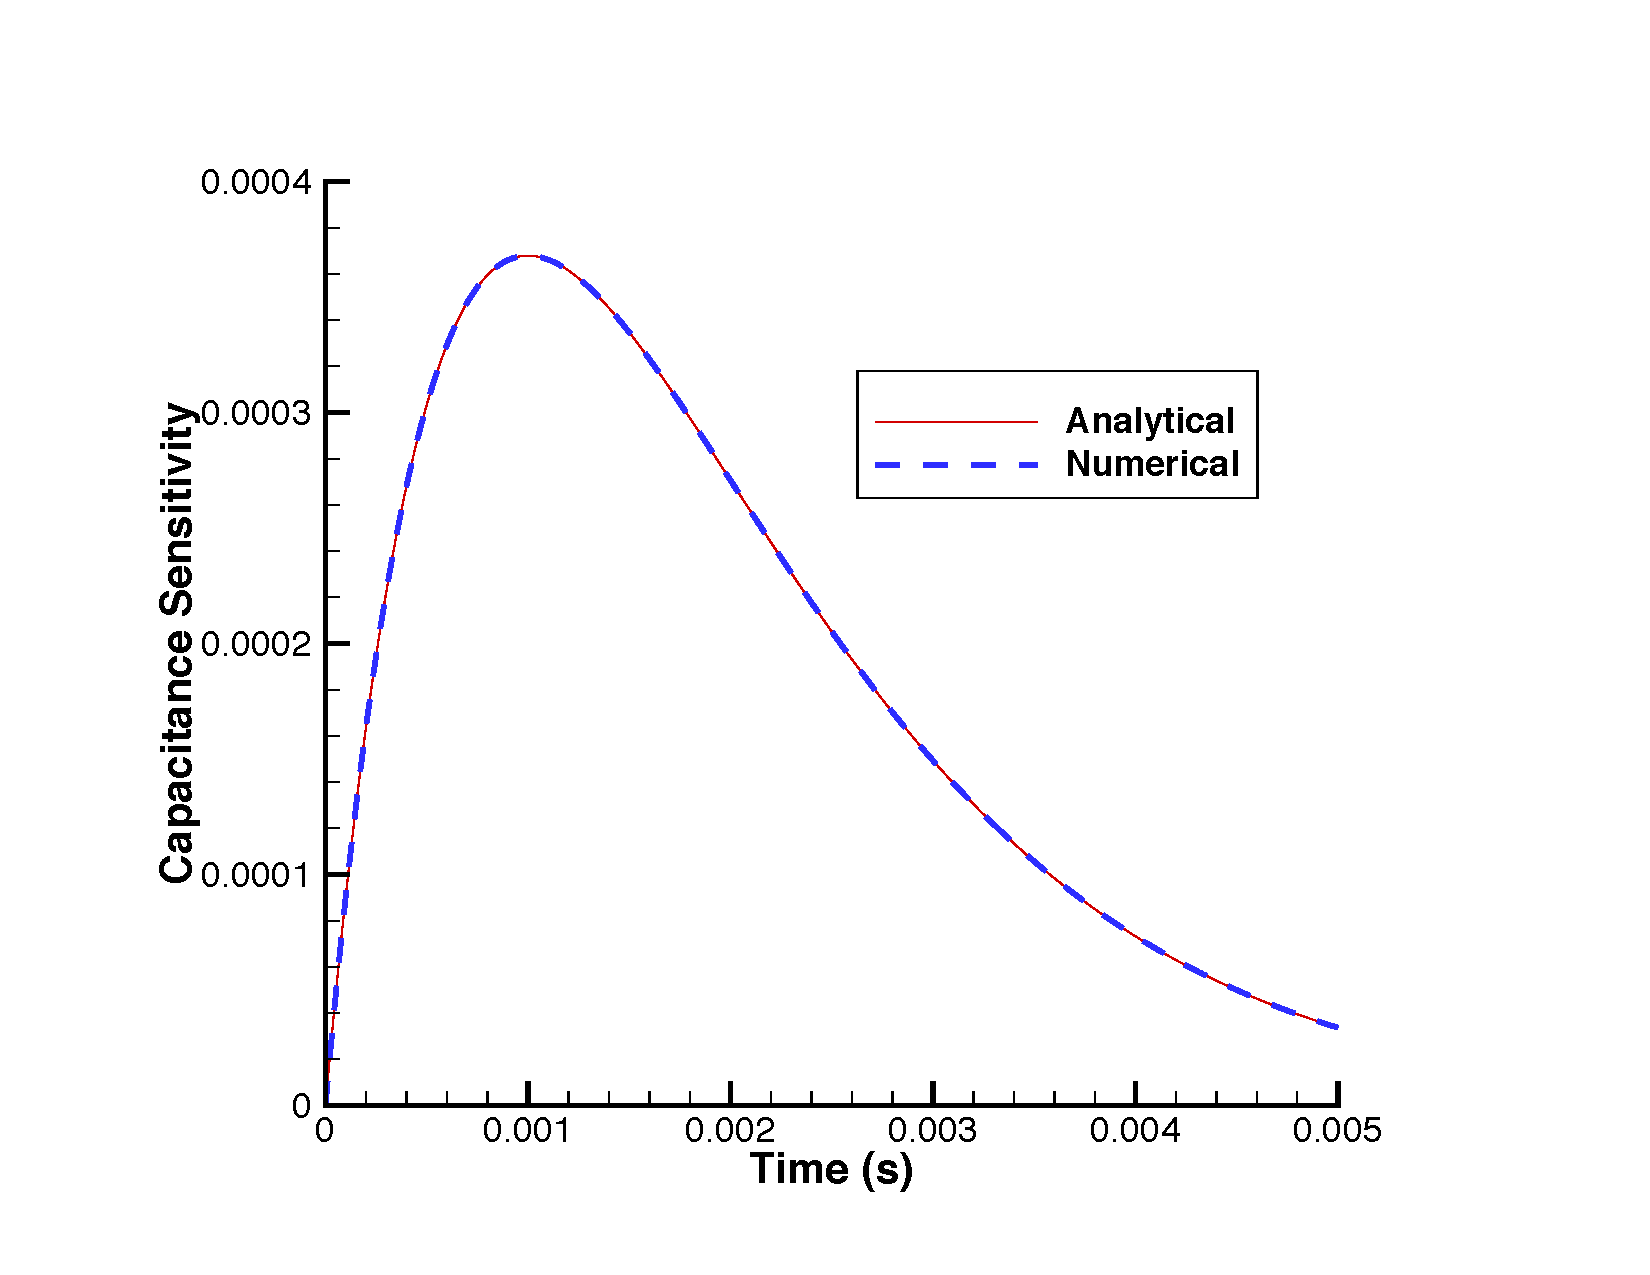
\includegraphics[]{sens}}
  \caption[Transient direct sensitivity result]
  {Transient direct sensitivity result.
\label{transientSensitivityResult}}
\end{figure}
Results for the transient example are given in figure~\ref{transientSensitivityResult}.
The analytic sensitivity solution is given by the solid line and the computed numerical
sensitivity is given by the dashed line.  The results match very well in this case,
with the two lines right on top of each other.

\clearpage
\subsubsection{Transient Adjoint Sensitivities}
Transient adjoint sensitivities are a good choice for really large numbers of 
parameters, and when the number of objective functions is modest.  For transient
calculations, each time point is considered a separate objective function, so it 
is best to use adjoints when the sensitivity of interest concerns only one or 
a handful of time points.

Set \texttt{direct=0 adjoint=1} to specify transient adjoint simulations.   The 
transient adjoint forumulation in \Xyce{} has similarities to the ones described
by Liu~\cite{Liu2014} and Meir~\cite{BLAST2012}.  An example netlist for a transient 
adjoint sensitivity
calculation is given in figure~\ref{Tran_Adjoint_Sensitivity_Netlist}.  This is a simple 
linear problem (RC driven by a sinewave), so it has an analytic solution.  
\begin{figure}[htbp]
  \begin{centering}
    \shadowbox{
      \begin{minipage}{0.9\textwidth}
        \begin{vquote}
\color{blue}*Test of transient adjoint sensitivities \color{black}
.param cap=1e-6
.param res=1e3

V1 1 0 0.0 sin (0.0 1.0 200 0.0 0.0 0.0 )
R1 1 2 {res}
C1 2 0 {cap}

.tran 1.0e-6 0.5e-2
.print tran format=tecplot V(1) V(2) 
.print TRANADJOINT format=tecplot

.options timeint method=gear reltol=1.0e-6 abstol=1e-6

\color{red}* Sensitivity commands
.SENS objfunc={V(2)} param=R1:R,C1:C
.options SENSITIVITY direct=0 adjoint=1\color{black}
.end
\end{vquote}
\end{minipage}
}
\caption[Adjoint Transient Sensitivity Example Netlist]
{Adjoint Transient Sensitivity Example Netlist \label{Tran_Adjoint_Sensitivity_Netlist} }
\end{centering}
\end{figure}
\begin{figure}[ht]
  \centering
  \scalebox{0.5}
  {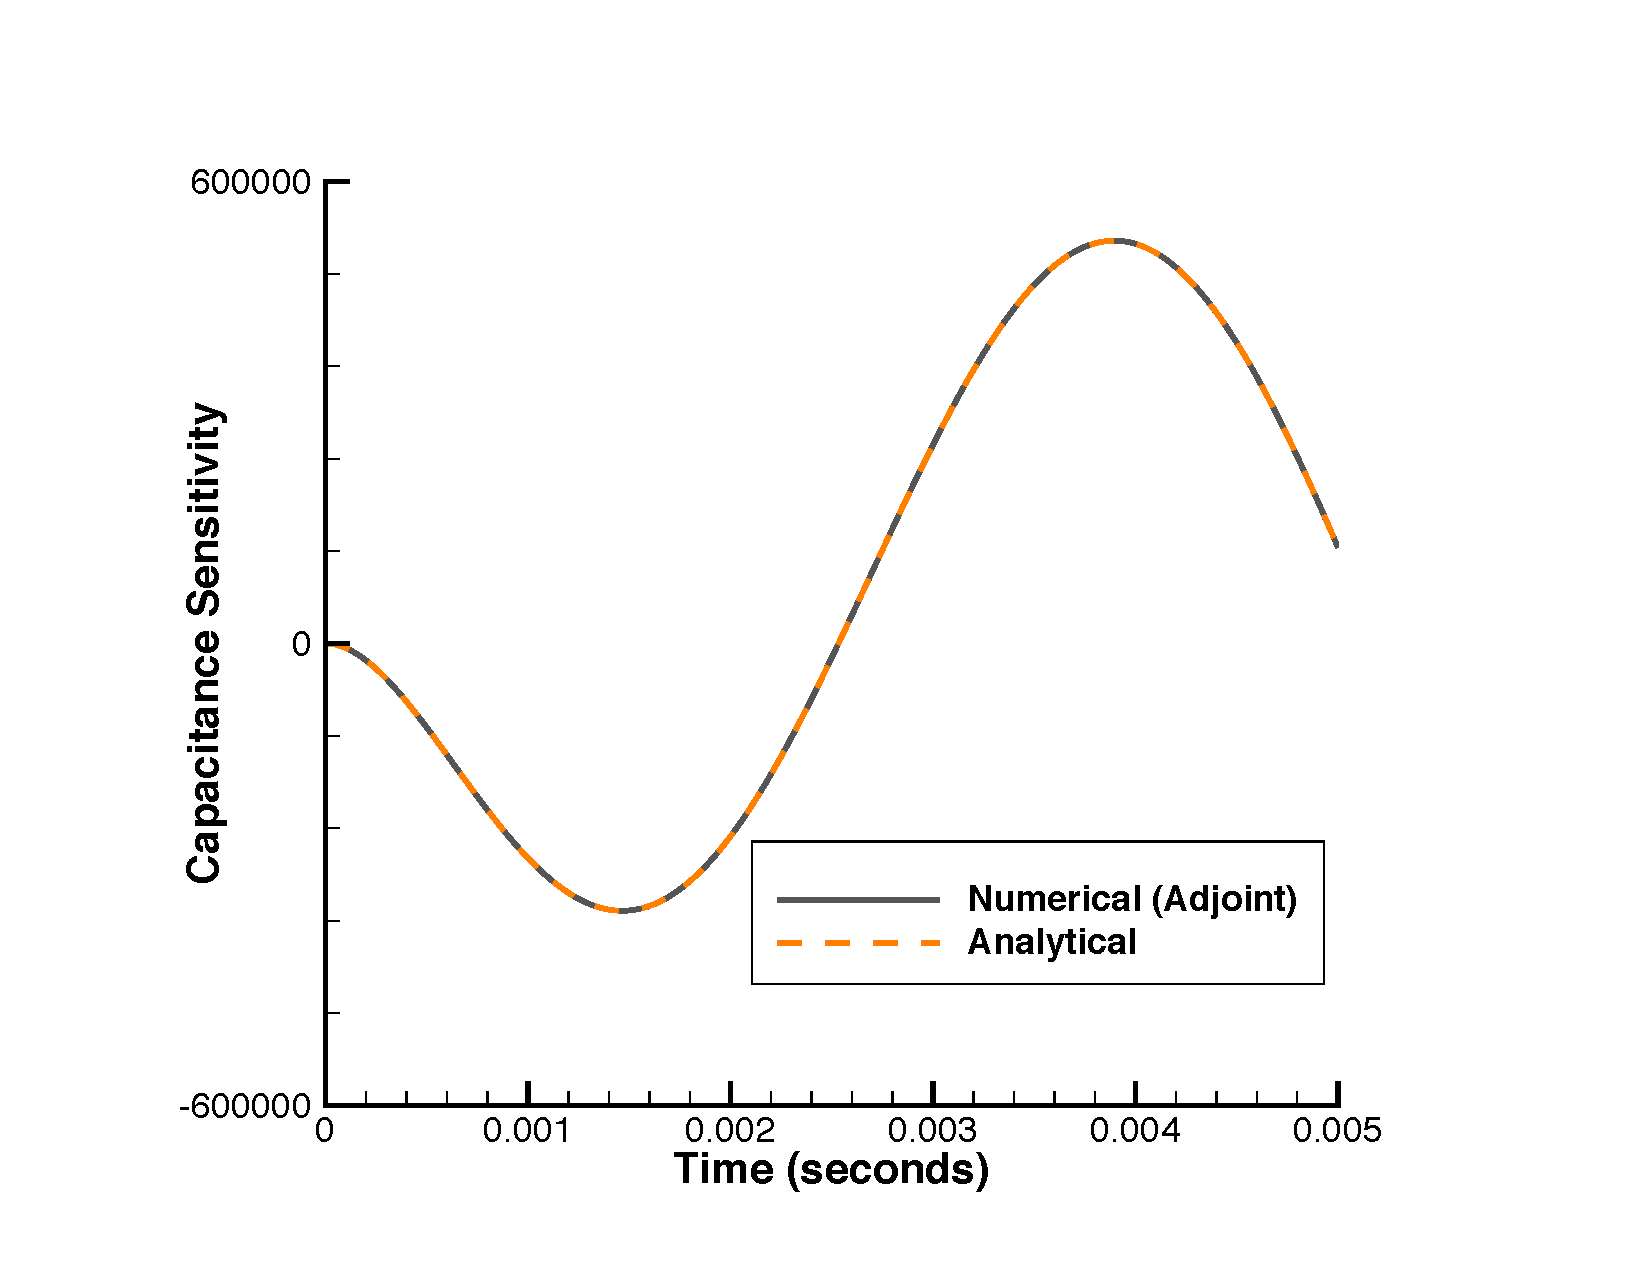
\includegraphics[]{sensCapGearAdj}}
  \caption[Transient adjoint sensitivity result]
  {Transient adjoint sensitivity result.
\label{transientAdjointSensitivityResult}}
\end{figure}
Results for the transient adjoint example are given in figure .
The analytic sensitivity solution is given by the dashed line and the computed numerical
sensitivity is given by the solid line.  The results match very well in this case,
with the two lines right on top of each other.

\clearpage
\subsection{AC Sensitivities}
Sensitivities can also be computed for small-signal AC analysis.  As with steady-state (DC) 
and transient analysis, both direct and adjoint sensitivities are supported.     An example
netlist which exercises the capability is shown in figure~\ref{AC_Sensitivity_Netlist}.

The netlist commands for AC sensitivities are very similar to those for DC, but with 
some small exceptions.   The expression library in \Xyce{} currently does not support
complex numbers, so the specification for objective functions is more limited.  As such, 
the \texttt{objfunc} parameter will not work with AC sensitivities, and the user should
instead specify outputs using \texttt{objvars} followed by a list of node names.  The
sensitivities that are computed will be for the voltages at the listed nodes, with respect
to the list of sensitivity parameters.
\begin{figure}[htbp]
  \begin{centering}
    \shadowbox{
      \begin{minipage}{0.99\textwidth}
        \begin{vquote}
\color{blue}*Lowpass filter test for AC sensitivities\color{black}
v1 1 0 ac 10.0
r1 1 2 4.7k
c1 2 0 47n

.ac dec 10 1 10k
.print ac  vm(1) vp(1) vm(2) vp(2)   
.print sens 

\color{red}* Sensitivity commands
.sens objvars=2 param=r1:r,c1:c
.options sensitivity direct=1 adjoint=0  stdoutput=1\color{black}
.end 
\end{vquote}
\end{minipage}
}
\caption[AC Sensitivity Example Netlist]
{AC Sensitivity Example Netlist \label{AC_Sensitivity_Netlist} }
\end{centering}
\end{figure}
For each specified output, there are four separate objective functions for
which sensitivities will be computed; magnitude and phase for the polar 
representation, as well as real and imaginary for the cartesian 
representation of the solution.   The console output for the example netlist,
for the first frequency, is shown in figure ~\ref{AC_Sensitivity_Result}.
\begin{figure}[htbp]
  \begin{centering}
    \shadowbox{
      \begin{minipage}{0.99\textwidth}
        \begin{vquote}

Direct Sensitivities for node V(2):
VR(2) = 1.0000e+01  VI(2) = -1.3880e-02
VM(2) = 1.0000e+01  VP(2) = -1.3880e-03

Name  Value Sensitivity\_Re  Sensitivity\_Im  Sensitivity\_Mag Sensitivity\_Phase
R1:R  4.7e+03  -8.1975e-09     -2.9531e-06     -4.0988e-09     -2.9531e-07
C1:C  4.7e-08  -8.1975e+02     -2.9531e+05     -4.0988e+02     -2.9531e+04

\end{vquote}
\end{minipage}
}
\caption[AC Sensitivity Example Result]
{AC Sensitivity Example Result\label{AC_Sensitivity_Result} }
\end{centering}
\end{figure}

\clearpage
\subsection{Output}
\label{SENS_Output}\index{\texttt{.PRINT}!\texttt{.SENS}}
For a full list and explanation of options related to \texttt{.SENS} output see 
the \Xyce{} Reference Guide\ReferenceGuide{}.

Sensitivity output can be sent to standard output, or to a user-specified
log file.  The format for this output is similar to that generated by the circuit
given in figure~\ref{DC_Sensitivity_Netlist}.
This feature is mainly made available in \Xyce{} so as to be similar to 
the sensitivity analysis of older circuit simulators.   However, for most uses 
it isn't the most practical output, so it is disabled by default.   To enable standard
output, one should set the following: 
\begin{verbatim}
.options SENSITIVITY STDOUTPUT=1
\end{verbatim}

In addition to the screen output, \Xyce{} can also produce a plottable file containing
all the requested sensitivities.  This file can be requested by adding either a \texttt{.PRINT SENS} 
or a \texttt{.PRINT TRANADJOINT} command to the input file.  Steady-state 
sensitivities (adjoint or direct) and transient direct sensitivities will be 
handled by the \texttt{.PRINT SENS} command.  Transient adjoint, on the other 
hand, is handled by the \texttt{.PRINT TRANADJOINT} command.

Unlike the traditional \texttt{.PRINT} line, both \texttt{.PRINT SENS} and \texttt{.PRINT TRANADJOINT} will
assume that the user wants all the sensitivities specified on the \texttt{.SENS} line.
As such it is not necessary (or possible) to specify specific sensitivities on the
\texttt{.PRINT SENS} line.  If the line exists, that is sufficient to produce
the file, and it will contain a column for every objective function and every
derivative.  The file name is the same as the one produced with 
\texttt{.PRINT}, but with  ``\texttt{.SENS}'' included just before the suffix.  
Similarly, for transient adjoint, the output file name has the string ``\texttt{.TRADJ}'' included before the suffix.
Note also, that most of the same output formats (\texttt{std}, \texttt{tecplot}, etc.) 
are available for \texttt{.PRINT SENS} and\texttt{.PRINT TRANADJOINT} as they are for conventional \texttt{.PRINT}.  The available
formats are listed in table~\ref{SENS_Output_table},~\ref{SENS_AC_Output_table}and~\ref{TRANADJOINT_Output_table}.
\begin{table}[htbp]
  \caption{Output generated for SENS analysis for .TRAN\label{SENS_Output_table}}
  \begin{tabularx}{\linewidth}{|p{2.75in}|Y|Y|}
    \rowcolor{XyceDarkBlue} \color{white}\textbf{Command} & \color{white}\textbf{Files} & \color{white}\textbf{Additional Columns} \\ \hline
\texttt{.PRINT SENS} & \emph{circuit-file}.SENS.prn & INDEX TIME \\ \hline
\texttt{.PRINT SENS FORMAT=GNUPLOT} & \emph{circuit-file}.SENS.prn & INDEX TIME \\ \hline
\texttt{.PRINT SENS FORMAT=SPLOT} & \emph{circuit-file}.SENS.prn & INDEX TIME \\ \hline
\texttt{.PRINT SENS FORMAT=NOINDEX} & \emph{circuit-file}.SENS.prn & INDEX TIME \\ \hline
\texttt{.PRINT SENS FORMAT=CSV} & \emph{circuit-file}.SENS.csv & TIME \\ \hline
\texttt{.PRINT SENS FORMAT=TECPLOT} & \emph{circuit-file}.SENS.dat & TIME \\ \hline
  \end{tabularx}
\end{table}
\begin{table}[htbp]
  \caption{Output generated for SENS analysis for .AC\label{SENS_AC_Output_table}}
  \begin{tabularx}{\linewidth}{|p{2.75in}|Y|Y|}
    \rowcolor{XyceDarkBlue} \color{white}\textbf{Command} & \color{white}\textbf{Files} & \color{white}\textbf{Additional Columns} \\ \hline
\texttt{.PRINT SENS} & \emph{circuit-file}.FD.SENS.prn & INDEX FREQ \\ \hline
\texttt{.PRINT SENS FORMAT=GNUPLOT} & \emph{circuit-file}.FD.SENS.prn & INDEX FREQ \\ \hline
\texttt{.PRINT SENS FORMAT=SPLOT} & \emph{circuit-file}.FD.SENS.prn & INDEX FREQ \\ \hline
\texttt{.PRINT SENS FORMAT=NOINDEX} & \emph{circuit-file}.FD.SENS.prn & INDEX FREQ \\ \hline
\texttt{.PRINT SENS FORMAT=CSV} & \emph{circuit-file}.FD.SENS.csv & FREQ \\ \hline
\texttt{.PRINT SENS FORMAT=TECPLOT} & \emph{circuit-file}.FD.SENS.dat & FREQ \\ \hline
  \end{tabularx}
\end{table}
As noted, transient adjoints are specified separately from \texttt{.PRINT SENS}.  
This is because the transient adjoint calculation is performed as a post-process, 
after the original forward calculation has been completed, and 
\Xyce{}'s forward outputters are no longer active.  To specify transient 
adjoint output, one must use \texttt{.PRINT TRANADJOINT} instead.  As it is 
possible to perform both a transient direct and a transient adjoint calculation 
as part of the same computation, and most of \Xyce{}'s output files are in 
column format, there wasn't an easy way to have them use the same outputter.
\begin{table}[htbp]
  \caption{Output generated for transient adjoint SENS analysis \label{TRANADJOINT_Output_table}}
  \begin{tabularx}{\linewidth}{|p{2.75in}|Y|Y|}
    \rowcolor{XyceDarkBlue} \color{white}\textbf{Command} & \color{white}\textbf{Files} & \color{white}\textbf{Additional Columns} \\ \hline
\texttt{.PRINT TRANADJOINT} & \emph{circuit-file}.TRADJ.prn & INDEX TIME \\ \hline
\texttt{.PRINT TRANADJOINT FORMAT=NOINDEX} & \emph{circuit-file}.TRADJ.prn & INDEX TIME \\ \hline
\texttt{.PRINT TRANADJOINT FORMAT=CSV} & \emph{circuit-file}.TRADJ.csv & TIME \\ \hline
\texttt{.PRINT TRANADJOINT FORMAT=TECPLOT} & \emph{circuit-file}.TRADJ.dat & TIME \\ \hline
  \end{tabularx}
\end{table}

\clearpage
\subsection{Notes about .SENS accuracy and formulation}
The sensitivity calculation in \Xyce{} is based on a chain rule calculation.   Ultimately,
the calculation will produce $dO/dp$, where $O$ is a user-specified objective function,
and $p$ is a user-specified parameter.  $dO/dp$ is equal to:
\begin{equation}
  \frac{dO}{dp} = \frac{\partial O}{\partial x}\frac{\partial x}{\partial p} + \frac{\partial O}{\partial p}
  \label{objectiveDerivative}
\end{equation}
\noindent where $x$ is a solution vector and $\partial x/\partial p$ is the sensitivity of that 
solution vector with respect to the parameter.  Evaluating~\ref{objectiveDerivative}
requires that $\partial x/\partial p$ be computed first.  The direct sensivity calculation for $\partial x/\partial p$ 
can be derived by considering the DAE form of the residual equation:
\begin{equation}
  F(x,t) = \dot{q}(x,t) + j(x,t) - b(t) = 0
  \label{residual}
\end{equation}
\noindent In this equation, $q$ represents quantities that must be differentiated 
with respect to time (such as capacitor charge), and $j$ represents algebraic 
terms that depend on the solution $x$ (such as DC currents), and $b$ are independent sources that 
only depend on time.  Equation~\ref{residual} is solved to obtain the solution, $x$.
To obtain sensitivities, one must differentiate this equation with respect to a 
parameter, $p$.
\begin{equation}
  \frac{dF}{dp} = \frac{d}{dp}\left( \dot{q} + j - b \right) = 0
  \label{dfdp}
\end{equation}
In steady-state, equation~\ref{dfdp} simplifies to:
\begin{equation}
  \frac{dF}{dp} = \frac{dj}{dp} - \frac{db}{dp} = 0
  \label{steady_dfdp}
\end{equation}
\noindent As $j$ is dependent upon $x$, the $\frac{dj}{dp}$ term must be expanded via chain rule, and
the resulting equation must be re-arranged to set up 
a matrix equation that can be solved to obtain $\frac{dx}{dp}$:
\begin{equation}
  \frac{dj}{dx}\frac{dx}{dp} = - \frac{dj}{dp} + \frac{db}{dp} 
  \label{finalSens}
\end{equation}
\noindent In equation~\ref{finalSens}, the terms on the right hand side are computed 
by the individual device models once the Newton loop the circuit analysis has 
converged.  The Jacobian matrix on the left hand side ($dj/dx$) is the same matrix 
used by the original analysis.  Once the linear system is solved, then $dx/dp$ is
available for the given parameter, and it can then be applied to equation~\ref{objectiveDerivative}.
For transient, a similar linear system is solved, which depends on the specific
time integration method used.  For Backward-Euler the linear system is:
\begin{equation}
  \left[ \frac{1}{h} \frac{dq}{dx} 
  + \frac{dj}{dx} \right] \frac{dx}{dp}_{n+1} 
 =
  -\frac{1}{h} \left[ \frac{dq}{dp}_{n+1} - \frac{dq}{dp}_n \right] 
 - \frac{dj}{dp} 
 + \frac{db}{dp} 
 + \frac{1}{h} \left[ \frac{dq}{dx} \right] \frac{dx}{dp}_n 
 \label{finalTransientSens}
\end{equation}
\noindent Where $h$ is the time step size.  As with ~\ref{finalSens}, the left hand side 
of the equation contains the original Jacobian matrix.

In general, the accuracy of the above calculation is dependent on the accuracy of the 
individual derivatives that comprise equations~\ref{objectiveDerivative} and~\ref{finalSens} 
or~\ref{finalTransientSens}.
In \Xyce{}, the Jacobian derivatives ($dj/dx$ and $dq/dx$) are always analytic.  Similarly, the
objective function derivatives ($dO/dx$) are also always analytic.  However, the derivatives
on the right hand side of~\ref{finalTransientSens} ($dj/dp$, $db/dp$ and $dq/dp$) depend on particular
device implementations.  If the device was implemented with analytic parameter sensitivies,
then those sensitivities are used.  If analytic derivatives were not available, then
the $dj/dp$, $dq/dp$ and $db/dp$ derivatives are computed using finite differences.  
A list of \Xyce{} devices, and which of them support analytic sensitivities, is given in the \Xyce{} Reference 
Guide\ReferenceGuide{}.

For some problems, finite difference derivatives will work fine, but some devices and/or circuit
problems have wide ranges of solution and/or parameter scalings, and this can render inaccurate 
finite difference derivatives.  As this capability develops, most devices should
eventually provide analytic derivatives.

The above derivation and arguments were given for direct sensitivities (as that is the only
form supported for both DC and transient), but the same 
ideas with regard to accuracy apply for adjoint sensitivites.

For transient, note that the transient direct calculation uses the same time steps 
that are used for the original circuit analysis.  It does not impose any additional error
control that is specific to the accuracy of $dx/dp$.

%%%%%%
% -------------------------------------------------------------------------
% S-parameter (.LIN) Analysis Section -------------------------------------
% -------------------------------------------------------------------------

\section{S-parameter Analysis}
\label{SP_Analysis}
\label{SP_Sweep_Overview}
\index{analysis!S-parameter} \index{S-parameter analysis} \index{\texttt{.LIN}}
\index{AC sweep} \index{analysis!AC sweep}

The S-parameter small-signal analysis of \Xyce{} computes linear transfer parameters as a
function of frequency for a general multi-port network. The program first computes the DC operating point of 
the circuit and then linearizes the circuit. The resultant linear circuit is then
analyzed over a user-specified range of frequencies. The output of a S-parameter
analysis is multi-port scattering (S) parameters. The S-parameters represent
the ratio of incident and scattered normalized voltage waves.  The analysis
results can also be output as Y-parameter or Z-parameter values.

\subsection{.LIN Statement}

One may specify S-parameter analyses by using a \verb|.LIN| command with a \verb|.AC| command in the netlist.
Here is an example of typical \verb|.AC| and \verb|.LIN| lines:

\Example{\\ 
\texttt{.AC DEC 10 1K 100MEG}  \\ 
\texttt{.LIN sparcalc=1 format=touchstone}  \\ 
}

The \verb|.LIN| analysis is similar to a basic small signal \verb|.AC| analysis, but it also calculates small signal 
transfer parameters between terminals identified using port (P) devices. The \Xyce{} Reference Guide\ReferenceGuide{} 
provides a complete description of \verb|.LIN| analysis and the P device.  To output Y-parameter
or Z-parameter values instead the \texttt{LINTYPE=Y} or \texttt{LINTYPE=Z} argument can be
used on the \texttt{.LIN} line.

\subsection{Port Devices}
\label{SP_Port}
\index{S-parameter analysis!port}

The \verb|.LIN| analysis computes the S-parameters based on the location of the port (P)
devices and the values of their reference impedances. The port devices identify
the ports used in \verb|.LIN| analysis. The \Xyce{} Reference Guide\ReferenceGuide{} 
provides a complete description of the port devices. Some examples are as follows:

\Example{\\   
%\texttt{*name nodelist type value  phase(deg)}  \\
\texttt{P1 1 0 port = 1} \\
\texttt{P2 12 0  port= 2  z0=100 }
}

NOTE:  Each port requires a unique port number. If a circuit has N ports, the netlist must
contain the sequential set of port numbers, 1 to N.  	

\subsection{Example}
An example S-parameter analysis netlist is given in figure~\ref{spExample}.  This example uses 2 ports.
The S parameters are outputted to a file in Touchstone 1 format \cite{touchstone2_std_2009}.
Touchstone 2 format is also supported.  Note that \texttt{SPARCALC=1} is specified on
the \texttt{.LIN} line.  If \texttt{SPARCALC=0} is specified instead then a \texttt{.AC}
analysis will be done.

\begin{figure}[htbp]
  \begin{centering}
    \shadowbox{
      \begin{minipage}{0.9\textwidth}
        \begin{vquote}
\color{blue}* S-parameter Analysis example\color{black}
P1 1 0 port= 1

C1 2 0 1e-2
Rgs 1 2 0.02

.subckt RCBlock IN OUT GND
R1 IN OUT 20
C1 IN OUT 1p
Cg1 OUT GND 1p
.ends

X1 2 3 0 RCBlock
X2 3 4 0 RCBlock
X3 4 5 0 RCBlock
X4 5 6 0 RCBlock
X5 6 7 0 RCBlock
X6 7 8 0 RCBlock
X7 8 9 0 RCBlock
X8 9 10 0 RCBlock
X9 10 11 0 RCBlock
X10 11 12 0 RCBlock

.AC DEC 10 10  1e5 

.LIN FORMAT=TOUCHSTONE  sparcalc=1

P2 12 0  port=2 z0=100

.END

\end{vquote}
\end{minipage}
}
\caption[S-parameter Example Netlist]
{S-parameter Example Netlist.  \label{spExample} }
\end{centering}
\end{figure}

\subsection{Output}
\label{LIN_Output}
For S-parameter analysis, the output is controlled by the \texttt{.LIN}
command when \texttt{SPARCALC=1} on that line.  Any information on
\texttt{.PRINT AC} lines will be ignored in that case.
Table~\ref{LIN_Output_table} lists the format options and files created.
If \texttt{SPARCALC=0} then a \texttt{.AC} analysis is done instead.

All three data formats defined in the Touchstone standard, which are real-imaginary (RI),
magnitude-angle(MA) and magnitude(db)-angle (DB), are supported.  The default is RI.
Other options can be selected via the inclusion of the \texttt{DATAFORMAT=<val>}
argument on the \texttt{.LIN} line. Per the Touchstone standard, all angle values
are output in degrees.

The default filename for both Touchstone formats is \texttt{<netlistName>.sNp}
where N is the number of ``ports'' (\texttt{P} devices) specified in the netlist.
The output can be redirected to another file with the \texttt{-o} command line
option or by using a \texttt{FILE=<filename>} argument on the \texttt{.LIN} line.

The default output is S-parameters.  The \texttt{LINTYPE=<S|Y|Z>} argument can be
used on the \texttt{.LIN} line to select Y-parameter or Z-parameter output instead.
(Note:  The default filename is still \texttt{<netlistName>.sNp} even if the
output file contains Y-parameter or Z-parameter output rather than S-parameter output.)
The \Xyce{} Reference Guide\ReferenceGuide{} has a complete listing of which
arguments, typically used on a \texttt{.PRINT} line also work on a \texttt{.LIN} line.

\begin{table}[htbp]
  \caption{Output generated for .LIN analysis \label{LIN_Output_table}}
  \begin{tabularx}{\linewidth}{|p{2.75in}|Y|Y|}
    \rowcolor{XyceDarkBlue} \color{white}\textbf{Command} & \color{white}\textbf{Files} & \color{white}\textbf{Format} \\ \hline
\texttt{.LIN} & \emph{circuit-file}.sNp & S-parameter data in Touchstone 2 format. Data format is RI. \\ \hline
\texttt{.LIN FORMAT=TOUCHSTONE} & \emph{circuit-file}.sNp & S-parameter data in Touchstone 1 format. Data format is RI. \\ \hline
\texttt{.LIN FORMAT=TOUCHSTONE2} & \emph{circuit-file}.sNp & S-parameter data in Touchstone 2 format. Data format is RI. \\ \hline
\texttt{.LIN DATAFORMAT=MA} & \emph{circuit-file}.sNp & S-parameter data in Touchstone 2 format. Data format is MA. \\ \hline
\texttt{.LIN DATAFORMAT=DB} & \emph{circuit-file}.sNp & S-parameter data in Touchstone 2 format. Data format is DB. \\ \hline
\texttt{.LIN LINTYPE=Y} & \emph{circuit-file}.sNp & Y-parameter data in Touchstone 2 format. Data format is RI. \\ \hline
\texttt{.LIN LINTYPE=Z} & \emph{circuit-file}.sNp & Z-parameter data in Touchstone 2 format. Data format is RI. \\ \hline

\texttt{\emph{Xyce} -r} & NA & This will produce a parsing error. \\ \hline
\texttt{\emph{Xyce} -r -a} & NA & This will produce a parsing error. \\ \hline

\end{tabularx}
\end{table}

When a \texttt{.LIN} analysis is done then additional output variable formats are available
via the \texttt{.PRINT AC} line, where \texttt{<index1>} and \texttt{<index2>} must both
be greater than 0 and also both less than or equal to the number of ports in the netlist:
\begin{XyceItemize}
\item \texttt{SR(<index1>,<index2>)} to output the real component of an S-parameter
\item \texttt{SI(<index1>,<index2>)} to output the imaginary component of an S-parameter
\item \texttt{SM(<index1>,<index2>)} to output the magnitude of an S-parameter
\item \texttt{SP(<index1>,<index2>)} to output the phase of an S-parameter in degrees
\item \texttt{SDB(<index1>,<index2>)} to output the magnitude of an S-parameter in decibels.
\item \texttt{YR(<index1>,<index2>)} to output the real component of a Y-parameter
\item \texttt{YI(<index1>,<index2>)} to output the imaginary component of a Y-parameter
\item \texttt{YM(<index1>,<index2>)} to output the magnitude of a Y-parameter
\item \texttt{YP(<index1>,<index2>)} to output the phase of a Y-parameter in degrees
\item \texttt{YDB(<index1>,<index2>)} to output the magnitude of a Y-parameter in decibels.
\item \texttt{ZR(<index1>,<index2>)} to output the real component of a Z-parameter
\item \texttt{ZI(<index1>,<index2>)} to output the imaginary component of a Z-parameter
\item \texttt{ZM(<index1>,<index2>)} to output the magnitude of a Z-parameter
\item \texttt{ZP(<index1>,<index2>)} to output the phase of a Z-parameter in degrees
\item \texttt{ZDB(<index1>,<index2>)} to output the magnitude of a Z-parameter in decibels.
\end{XyceItemize}

\Example{\\
\texttt{.print AC SR(1,1) YI(1,2) ZM(2,1)}
}

%%% Local Variables:
%%% mode: latex
%%% End:
% END of Xyce_UG_ch09.tex ************
